\status{review}
\chapter{Scintillators in muEDM}
\label{ch:muEDM:entrance}
\begin{refsection}

{\itshape
In the previous chapter, the muEDM experiment was introduced and the current status was described.
In this, we will describe the simulations and beamtimes connected to few items of this experiment: entrance detector, the TOF measurement and the beam monitor. 
We will start with the \gf simulations of thin and thick scintillators, moving then to the entrance detector and the `telescope' used in the beamtime of 2022. 
After that the TOF detector.
We will then move through the beamtimes.
}

\status{review}
\section{Short intro to scintillators}
\label{sec:muEDM:scintillators}
    A \textit{scintillator} is any material that emits light when exposed to ionizing radiation, like high-energy photons or charged particles.
    The main distinction is between organic and inorganic scintillators:
    \begin{outline}
        \1 Organic scintillators are typically composed of carbon, hydrogen, and other organic (carbon-based) compounds. These materials often include fluorescent dyes or organic molecules that emit light when excited by ionizing radiation.
        They are often used for neutron detection and can also be used for other types of radiation, such as alpha and beta particles. They are versatile and find applications in various fields, including nuclear and particle physics
        \1 Inorganic scintillators are composed of inorganic materials that do not primarily contain carbon-hydrogen (C-H) bonds. These materials can include compounds like sodium iodide (\ce{NaI(Tl)}), cesium iodide (\ce{CsI(Tl)}), bismuth germanate (\ce{Bi4Ge3O12} often "BGO"), and lanthanum halides (\ce{LaBr3} and \ce{LaCl3}).
        These are commonly used in applications requiring high energy resolution and efficiency, like in gamma-ray spectroscopy, high-energy physics experiments, or medical imaging.
    \end{outline}
    Organic scintillators typically have relatively fast response times and are less expensive, while inorganic scintillators tend to have better energy resolution.
    Organic scintillators dived in: liquid, crystaline and plastic.
    We will discuss plastic scintillators. 
    An example of a liquid scintillator, based on Xenon, will be presented when describing the MEG II apparatus (see Ch.\ref{ch:MEG}).

    \status{review}
    \subsection{Plastic scintillators}
        Plastic scintillators are by far the most widely used and their densities range from $1.03$ to $\SI{1.2}{g\per cm^3}$, with a light yield of $1\divisionsymbol\SI{100}{\upgamma/eV}$ of energy deposit \cite{PDG}.
        The number of photons emitted is not linear with the energy deposit: in very dense ionization the light yield is lower than expected.
        This effect is described with the Birks's formula (Eq.~\ref{eq:Birk}) for the luminescence $\mathcal{L}$.
        \begin{equation}
            \dv{\mathcal{L}}{x} = \mathcal{L}_0 \frac{\dv{E}{x}}{1 + k \dv{E}{x}}
            \label{eq:Birk}
        \end{equation}
        Where $\dv{\mathcal{L}}{x}$ is the Light output, $\dv{E}{x}$ the energy loss per unit length by ionizing radiation and $k$ Birks' constant (also known as the stopping power ratio).\\
        Plastic scintillators are widely used in particle detectors due to their high light yield and fast response time, enabling sub-nanosecond timing resolution. 
        They offer the advantage of pulse shape discrimination, allowing for particle identification based on emitted light during the decay "tail".
        These are also popular due to their ease of fabrication into various shapes and cost-effectiveness. 
        Scintillating fibers made from plastic scintillators are commonly used in tracking and calorimetry applications.

    \status{review}
    \subsection{Scintillating Fibers}
        This is also a good moment to introduce The concept of \textit{scintillating fibers}.
        We will not use them in this chapter but will be key in Ch.~\ref{ch:muEDM:tracker}, dedicated to the $\Ae$ tracking.\\
        A fiber is generally a thin plastic scintillator that undergoes a process named \textit{cladding}.
        This process consists of covering the thin structure with multiple layers of lower refractive index, which helps to trap the scintillation light in the \textit{core} of the fiber.
        Scintillating fibers (SciFi) have become quite common due to their speed, density, radiation resistance, and resolution. 
        At the same time, SciFi trackers can handle high rates and radiation. 
        The downside of this technology is the requirement for sensitive photodetectors, due to low photon yield at the fiber's end. 

        \noindent
        Another interesting aspect is that it is possible to control the sensitive region by pairing scintillating and non-scintillating fibers. 
        This results in a loss in the collected light but allows the extraction of the light produced in specific regions without creating unwanted hits.
        On this point is important to remember that the particles will still interact with the non-scintillating fiber, losing energy and undergoing multiple scattering.
        A careful balance is required.

        \paragraph{Typical Fibers}
        The typical material for the core is a polystyrene-based scintillator or Wave-Length Shifter (refractive index $n\approx1.59$) while the cladding is often of PMMA\footnote{Poly(methyl methacrylate) is a synthetic polymer which goes by many names: acrylic glass, plexiglas, lucite, ...} ($n\approx1.49$), sometimes followed by an additional fluorinated PMMA cladding ($n\approx1.42$) for enhanced light capture. 
        The resulting diameter is of the order of few $\SI{0.1}{mm}$.
        The fraction of the light transported is around 6\% for single-clad fibers and 10\% for double-clad fibers. 
        Considering concrete numbers: a minimum-ionizing particle in 1 mm diameter fiber would generate a few thousand photons.
        The number of these reaching the ends of the fiber depends on the length and the \textit{attenuation length} but goes from a few hundred to a few photons.
        The attenuation length, the distance over which the signal diminishes to 1/e of its original value, is influenced by factors such as re-absorption of emitted photons, polymer base crystallinity, photodetector sensitivity, and internal surface quality. 
        High-quality fibers can achieve attenuation lengths of several meters.
        In case the quality of the fiber is not enough for the task at hand, the addition of a very thin layer (few atoms) of a reflective material, like aluminum, can further improve the light collection. 

    \status{review}
    \subsection{Scintillation process}
        Charged particles passing through matter create excited molecules, some of which release a small amount of their energy as optical photons through a process known as scintillation. This phenomenon is prominent in organic substances containing aromatic rings like polystyrene (PS) and polyvinyltoluene (PVT), as well as in liquids such as toluene, xylene, and pseudocumene.\\
        In fluorescence, molecules are initially excited by absorbing a photon and then deexcite by emitting a longer wavelength photon. To shift scintillation light to a more convenient wavelength, fluorescent materials are used as ``wave-shifters''.
        However, complex molecules in fluorescence can exhibit self-absorption, which shortens the attenuation length. 
        The greater the difference between absorption and emission wavelengths (Stokes' shift), the less self-absorption occurs, making a larger shift desirable.\\
        
        \noindent
        In high-energy physics, plastic scintillators are typically composed of selected fluors dissolved in a plastic base containing aromatic rings. Most plastic scintillators use either PVT or PS as their base, with PVT-based scintillators being often brighter. 
        Adding a fluor in high concentration (1\% by weight) into the base helps improve the attenuation length, as it efficiently re-radiates absorbed energy at wavelengths where the base is more transparent.
        The primary fluor also plays a crucial role in shortening the scintillator's decay time, increasing the total light yield. 
        The strong coupling between the base and fluor, known as Foerster resonance energy transfer, occurs at short distances, enhancing the speed and light yield of plastic scintillators.
        In some cases, a "secondary" fluor may be added in fractional percent levels, and occasionally even a third.
        External wavelength shifters are employed to aid light collection in complex geometries. They consist of a lightpipe with a wave-shifting fluor dissolved in a non-scintillating base. Typically, an acrylic base is used for its optical qualities, along with a single fluor to shift the emitted light to the blue-green range. These shifters also contain additives to absorb ultraviolet light and reduce sensitivity to Cherenkov radiation.
        \noindent
        For specialized applications, scintillators with increased radiation resistance or unique properties like neutron/gamma discrimination can be created by significantly increasing fluor concentrations.
        
\status{review}
\section{\gf simulations}
    \label{sec:muEDM:entrance:sim}
    \status{review}
    \subsection{What is \gf?}
        \gf (GEometry ANd Tracking) is a powerful open-source simulation toolkit used in various scientific fields, primarily for studying the interactions of particles with matter, and is widely employed in particle, nuclear, and medical physics. 
        At its core, \gf works by representing the physical world as a set of geometric shapes and materials. 
        After defining the properties of particles, their energy, and the materials they interact with, \gf simulates their behavior. 
        This toolkit utilizes a range of physics models and algorithms to accurately model particle interactions, including electromagnetic, hadronic, and optical processes. It can simulate particles of various energies, from subatomic to cosmic ray levels.
        The simulation is \textit{step} based: at every interaction, the physical properties of the particle are updated and, if needed, secondary particles are generated. 
        Steps are forced to end when crossing the boundary between two materials/volumes to ensure proper care is taken in the transition. 
        This is of particular importance for optical simulations, such as the propagation of OpticalPhotons produced by scintillation.

    \status{review}
    \subsection{Entrance system}
        To study the feasibility of the entrance thin scintillator, a \gf simulation was developed.
        The first step, after achieving a running simulation of scintillation, was to study the range of muons of the interesting momenta, as well as the energy deposit. 
        These first results are shown in Fig.~\ref{fig:muEDM:entrance:edep}.
        Here we can see the energy deposit for $\Ae$ and $\Am$ in scintillators of different thicknesses, reflecting the well-known Bethe-Bloch plot shown in Fig.~\ref{fig:muEDM:entrance:BetheBloch}. 
        Interesting features are:
        \begin{outline}
            \1 The energy deposit is linear with the thickness for the $\Ae$
            \1 The linearity is lost for the $\Am$. First, we have an exponential trend and then a plateau, when $E_{dep}\approx E_k$ and the $\Am$ is stopped
            \1 The shape of the deposit slowly changes from Landau to Gaussian
        \end{outline}
        In Fig.~\ref{fig:muEDM:entrance:edep:log} we recover the linear (and then exponential) trend when sampling the energy deposit for $\Am$ for lower thicknesses at both \SI{28}{MeV/c} and \SI{128}{MeV/c}.


        \begin{figure}
            \centering
            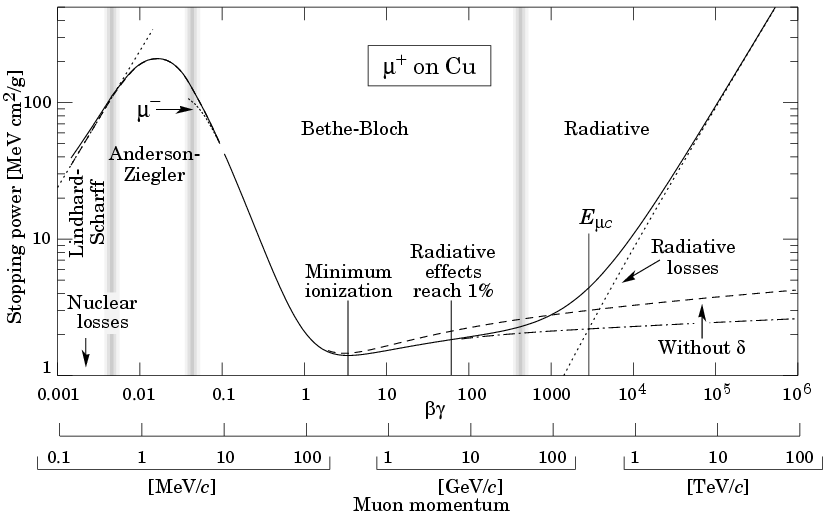
\includegraphics[width=0.9\textwidth]{Figures/muEDM/Entrance/BetheBloch.png}\\
            \caption{This figure illustrates the Bethe-Bloch formula \cite{PDG}, a vital tool in particle physics, depicting how charged particles lose energy when traversing through matter.}
            \label{fig:muEDM:entrance:BetheBloch}
        \end{figure}
        
        \begin{figure}   
            \centering
            \subfloat[A \SI{28}{MeV\per c} $\Ae$ has $E_k \approx \SI{27.5}{MeV}$.]{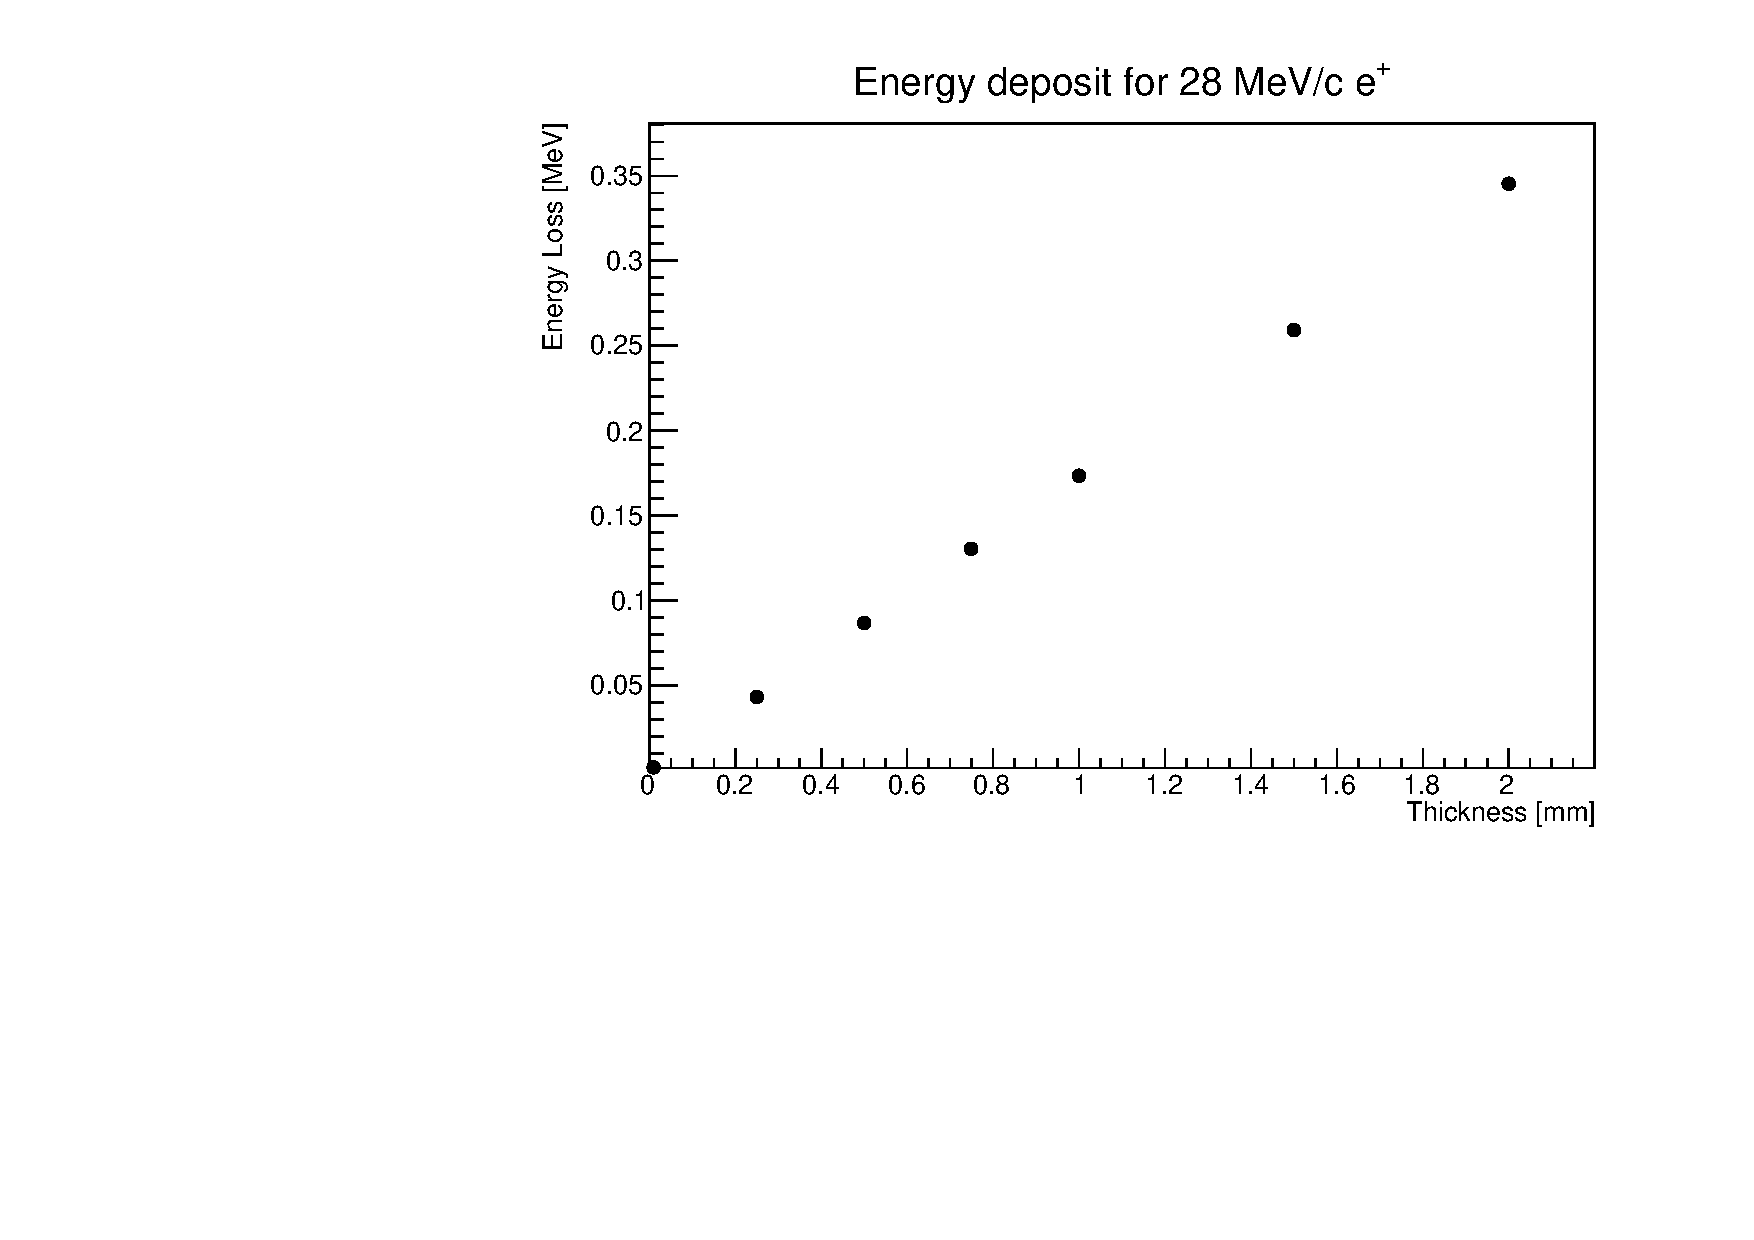
\includegraphics[height=5.5cm, keepaspectratio]{Figures/muEDM/Entrance/e_28_thick.pdf}\label{fig:muEDM:entrance:edep:e28}}
            \hfill
            \subfloat[Landau energy deposit for the positrons.]{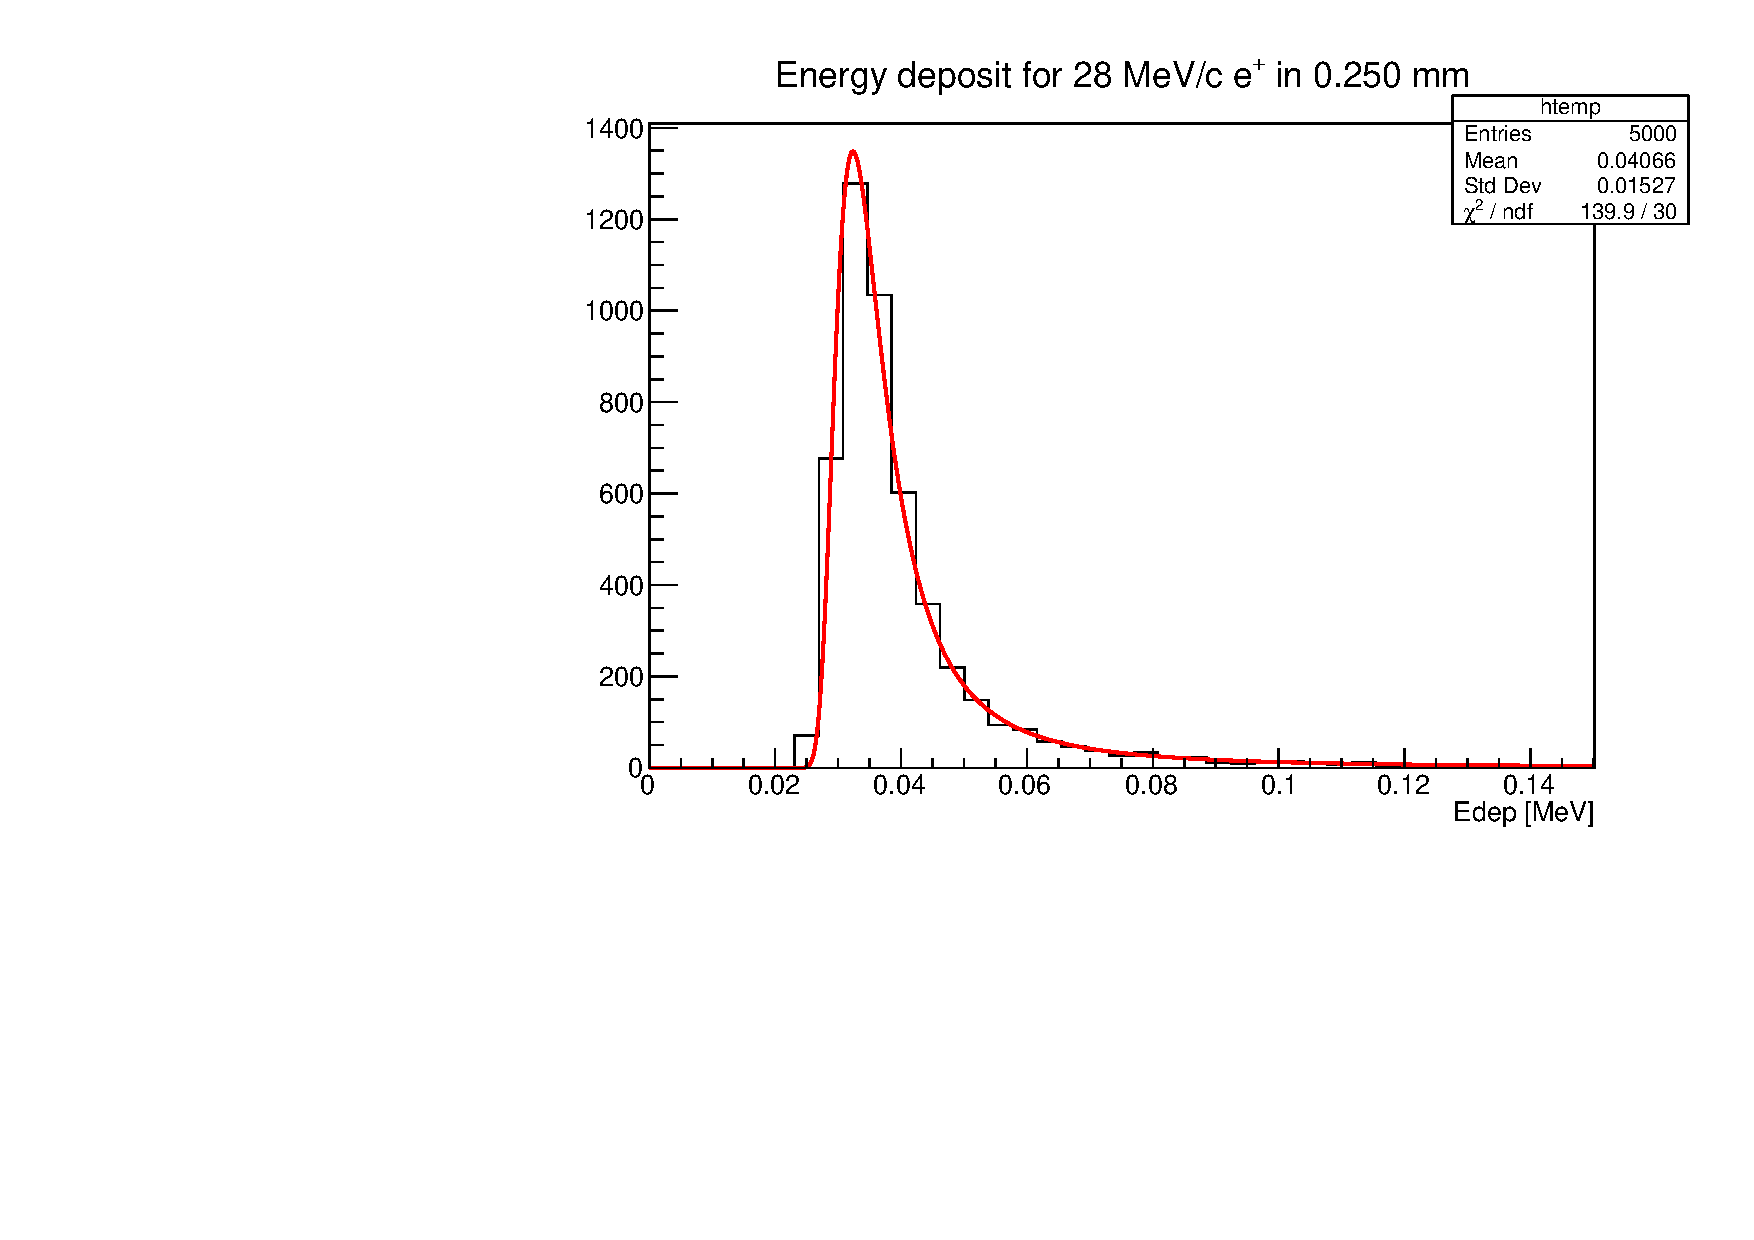
\includegraphics[height=5.5cm, keepaspectratio]{Figures/muEDM/Entrance/e_28_Edep_0.250.pdf}\label{fig:muEDM:entrance:edep:e28_0.25}}\\
            \subfloat[A \SI{28}{MeV\per c} $\Am$ has $E_k \approx \SI{3.6}{MeV}$.]{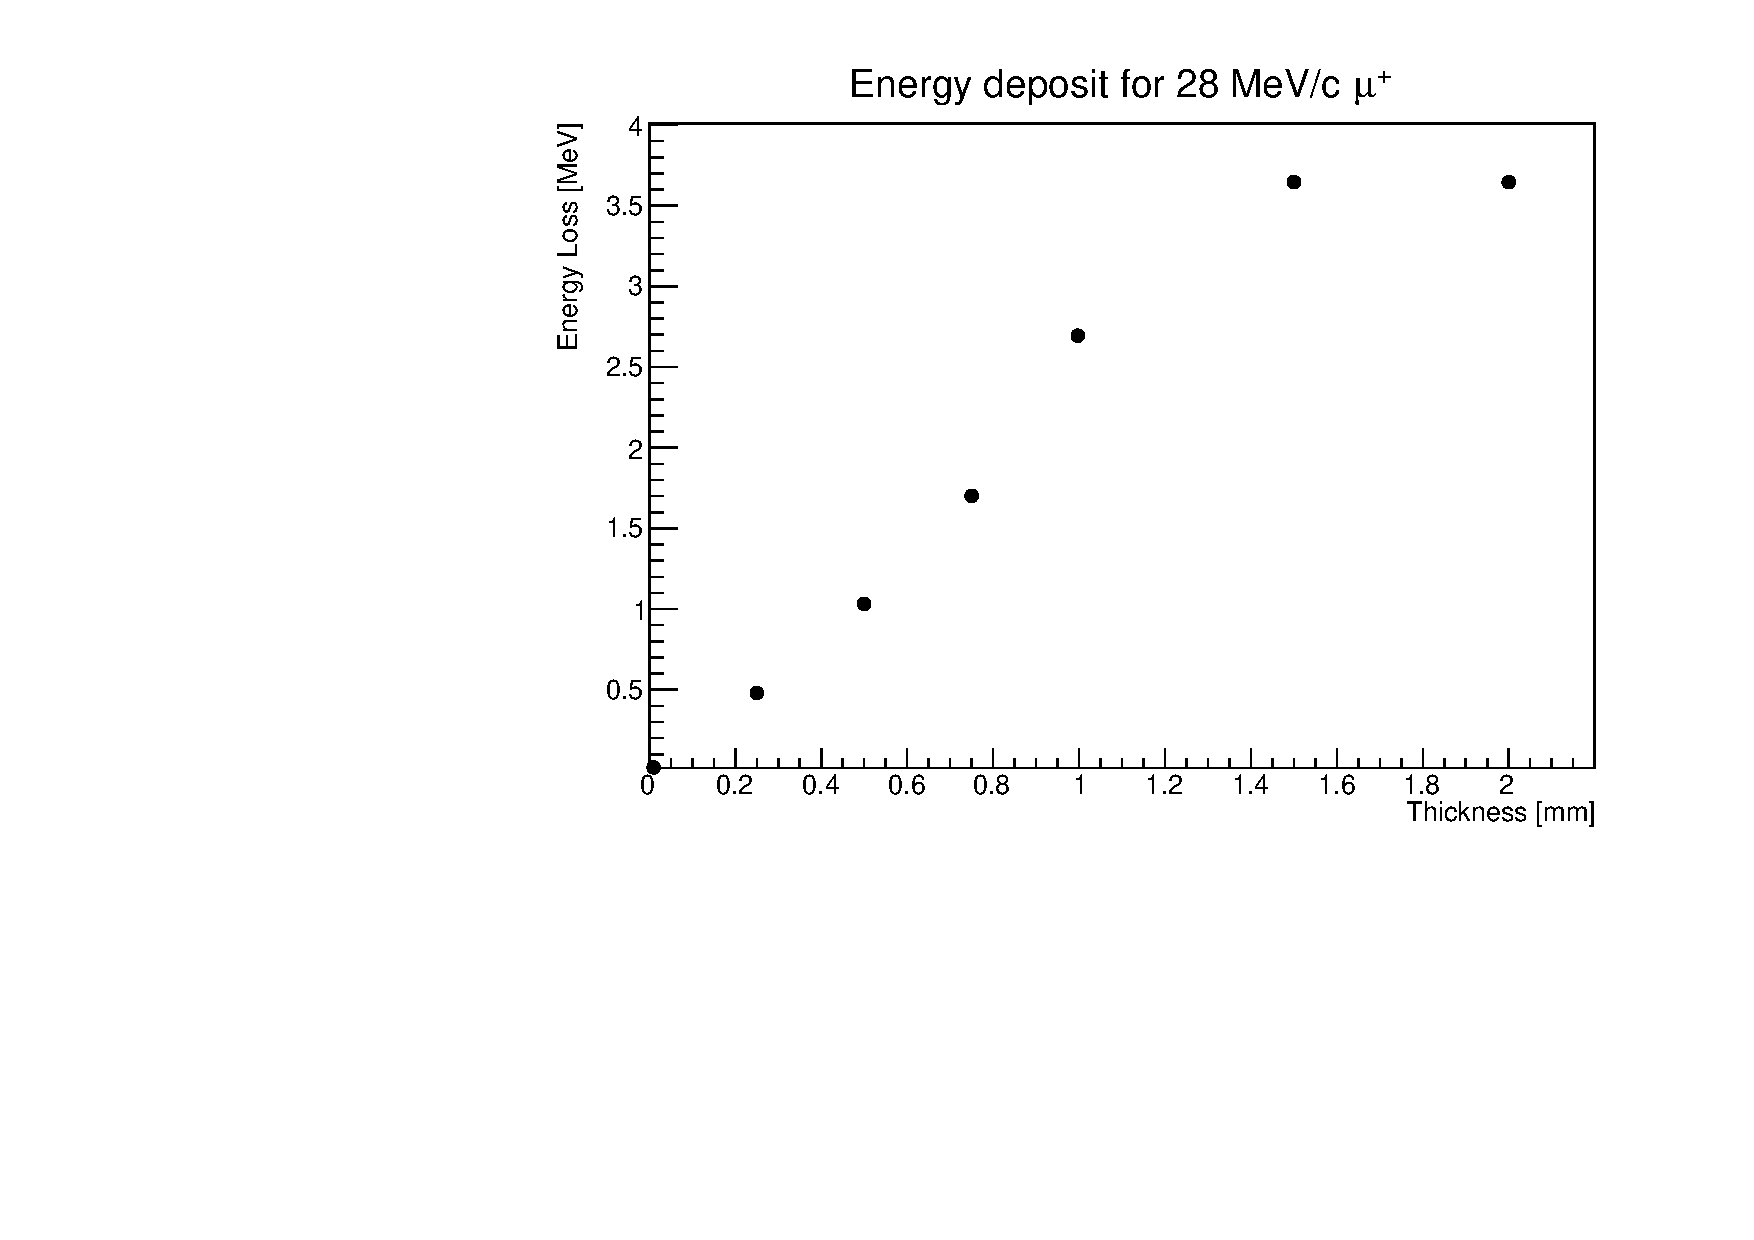
\includegraphics[height=5.5cm, keepaspectratio]{Figures/muEDM/Entrance/mu_28_thick.pdf}\label{fig:muEDM:entrance:edep:mu28}}
            \hfill
            \subfloat[The energy deposit slowly moves from Landau to a gaussian distribution.]{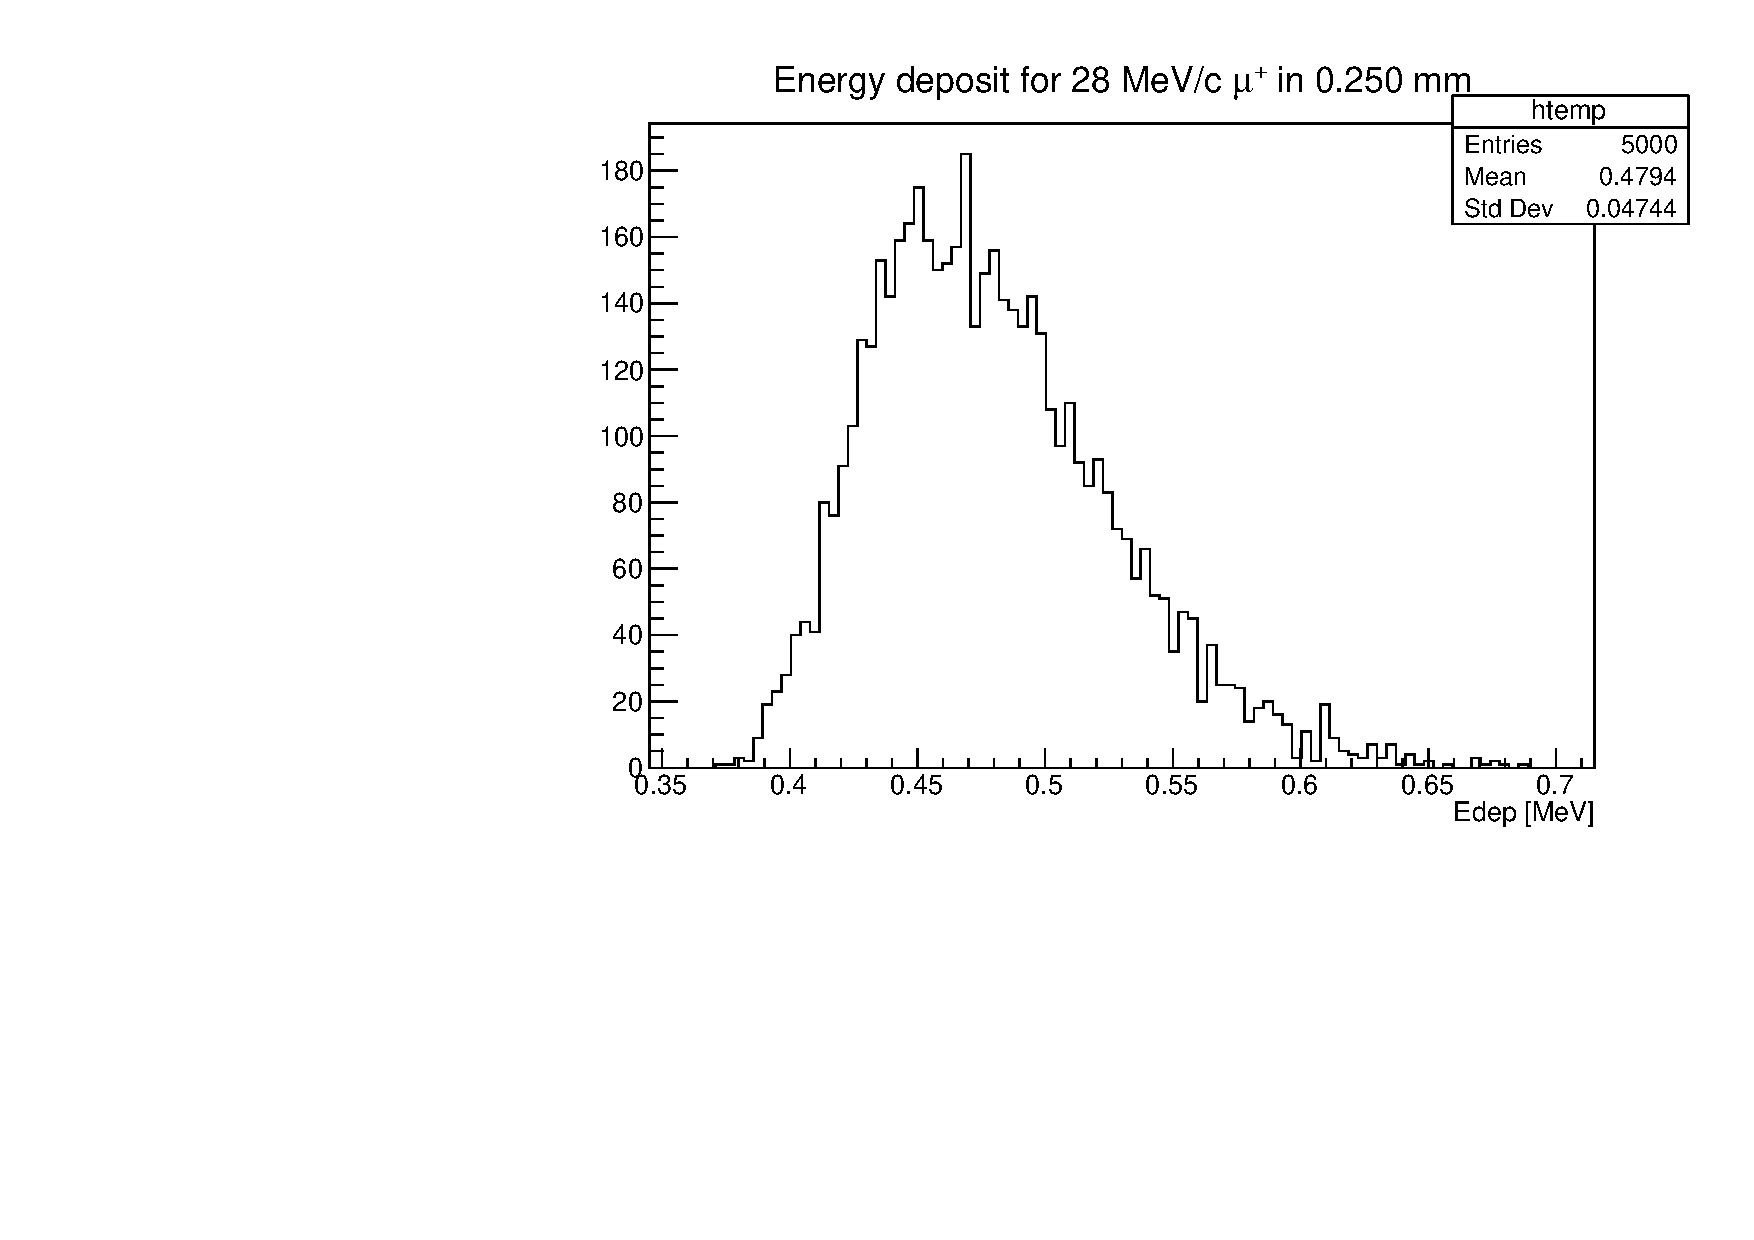
\includegraphics[height=5.5cm, keepaspectratio]{Figures/muEDM/Entrance/mu_28_Edep_0.250.pdf}\label{fig:muEDM:entrance:edep:mu28_0.25}}
            \caption{Curve for the average energy deposit in a \bc{400} scintillator for $\Am$ (\ref{fig:muEDM:entrance:edep:e28}) and $\Ae$ (\ref{fig:muEDM:entrance:edep:mu28}) at \SI{28}{MeV\per c}. Clearly visible is the linearity of the energy loss for the $\Ae$ with thickness. This linearity is lost for the $\Am$: first, we see an exponential trend and then a plateau when $E_{dep}\approx E_k$ and the $\Am$ is stopped. The distribution of the energy deposit slowly transitions from a Landau to a Gaussian: (\ref{fig:muEDM:entrance:edep:e28_0.25}) is an example of the first type; (\ref{fig:muEDM:entrance:edep:e28_0.25}) is an example of the transition.}
            \label{fig:muEDM:entrance:edep}
        \end{figure}
        
        \begin{figure}   
            \centering
            \subfloat[A \SI{28}{MeV\per c} $\Am$ has $E_k \approx \SI{3.6}{MeV}$.]{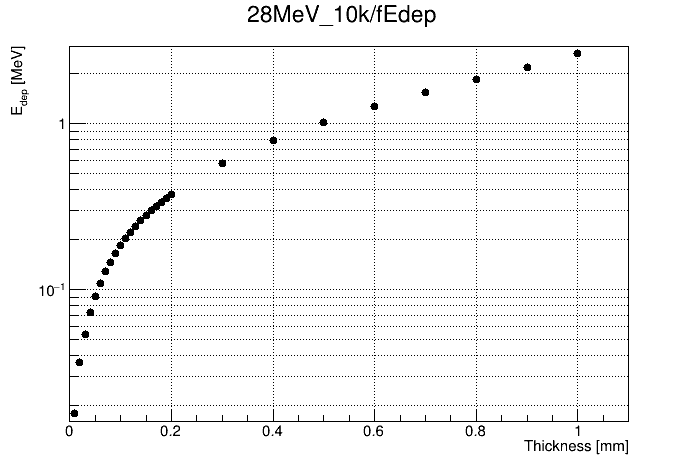
\includegraphics[height=5.5cm, keepaspectratio]{Figures/muEDM/Entrance/28mu_edep.png}\label{fig:muEDM:entrance:edep:log:28}}
            \hfill
            \subfloat[A \SI{128}{MeV\per c} $\Am$ has $E_k \approx \SI{60.3}{MeV}$.]{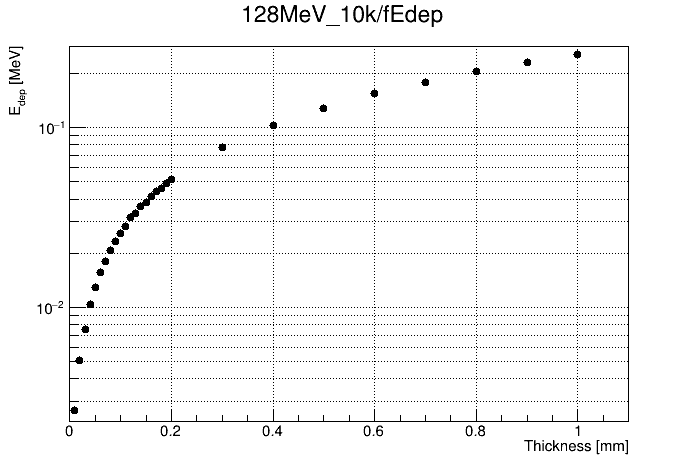
\includegraphics[height=5.5cm, keepaspectratio]{Figures/muEDM/Entrance/128mu_edep.png}\label{fig:muEDM:entrance:edep:log:128}}
            \caption{Detail on the lower section of the curve for the average energy deposit in a \bc{400} scintillator for $\Am$ at \SI{28}{MeV\per c} and \SI{128}{MeV\per c}.}
            \label{fig:muEDM:entrance:edep:log}
        \end{figure}

        \subsubsection{Multiple scattering}
            An important sanity check was also to study the multiple scattering in the scintillator. 
            More details on the functional description and the \gf implementation of the multiple scattering will follow, in \ref{sec:muEDM:tim}.
            This was done with a fit to the Highland formula (Eq.~\ref{eq:highland}) the average value of the scattering angle as a function of the thickness. 
            These fits are shown in Fig.~\ref{fig:muEDM:entrance:ms} and the results, $X_{0, 28MeV} = \SI{54.36(17)}{gm/cm^2}$ and $X_{0, 128MeV} = \SI{54.30(14)}{gm/cm^2}$, are consistent with the value for \bc{400} of $X_{0}\sim 50$.

        \subsubsection{Thickness and number of photons}
            The amount of energy deposited by the incoming particle is reflected by the number of photons generated by scintillation.
            These photons scatter inside the scintillator until they arrive on the external surface.
            Not all photons produced will be detected.
            This is affected by the position, number, size, and PDE\footnote{Photon detection efficiency describes the effectiveness of a photon detector in registering incoming photons. It quantifies the probability that a photon incident on the detector will be detected and converted into an electrical signal} of the SiPMs. 
            To simulate the SiPM readout we can use a silicon volume coupled to the scintillator via an additional volume of optical grease\footnote{Also known as optical coupling grease or index-matching grease, is a specialized type of grease used in optics and photonics applications. It is designed to improve the optical coupling between optical components.}.
            The first iteration was performed in a perfect scenario, with a floating scintillator glued to the sensors.
            The second iteration matches reality more, and a light guide is used to hold the scintillator and give enough surface for the SiPM gluing.
            In Fig.~\ref{fig:muEDM:entrance:guide} the total number of produced optical photons is compared to the number of photons collected with/without an optical guide.
            A few points are worth underlying:
            \begin{outline}
                \1 There is a drop in the number of photons arriving at the sensors, as expected
                \1 The number of photoelectrons is further reduced by the PDE (20\% $\divisionsymbol$ 40\%) of the SiPM
                \1 Number and size of the SiPM active region plays a big role (here 16 SiPMs were used)
                \1 The position of the SiPM on the edges is less influential than what naively might be expected. The photon distribution is quite uniform once the scintillator size is $\sim$cm
            \end{outline}
            Looking at Fig.~\ref{ffig:muEDM:entrance:guide:28mu}, the number of expected photoelectrons per SiPM for interesting thicknesses is around $(\SI{50}{\micro\meter}, \sim10\ \gamma)\divisionsymbol(\SI{200}{\micro\meter}, \sim30\ \gamma)$.
            At the same time, the dark rate count limits how low the thresholds can be set in a real setup.
            Multiple readouts would allow us to lower the threshold and improve the dark noise rejection. Calling the sides $s_i$, options could be $(s_1\land s_3)\lor(s_2\land s_4)$, $(s_1\land s_3)\land(s_2\land s_4)$, or simply $(s_1\land s_3)$.
            We studied these different readouts schemes in the beamtime of Dec. 2023 (see Sec.~\ref{sec:muEDM:beamtime2023}) 
            \begin{figure}   
                \centering
                \subfloat[A \SI{28}{MeV\per c} $\Am$ has $E_k \approx \SI{3.6}{MeV}$.]{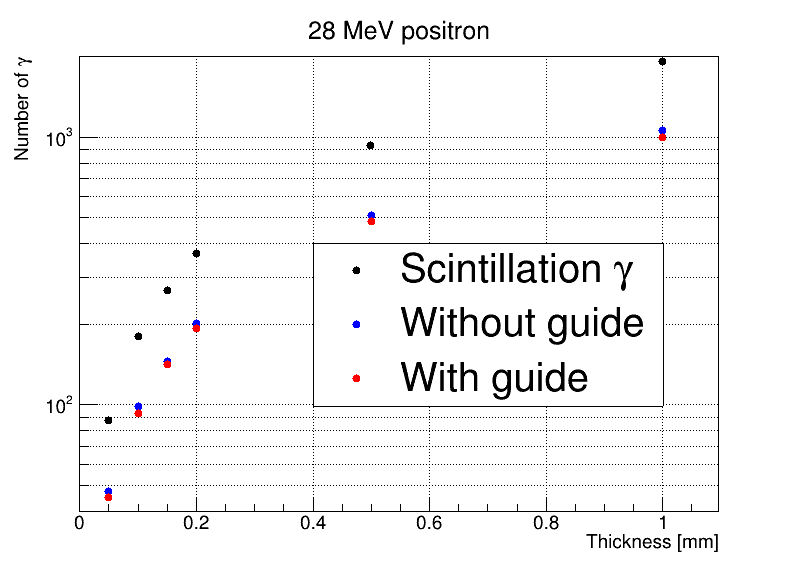
\includegraphics[height=5.5cm, keepaspectratio]{Figures/muEDM/Entrance/28e_guide.png}\label{fig:muEDM:entrance:guide:28e}}
                \hfill
                \subfloat[A \SI{128}{MeV\per c} $\Am$ has $E_k \approx \SI{60.3}{MeV}$.]{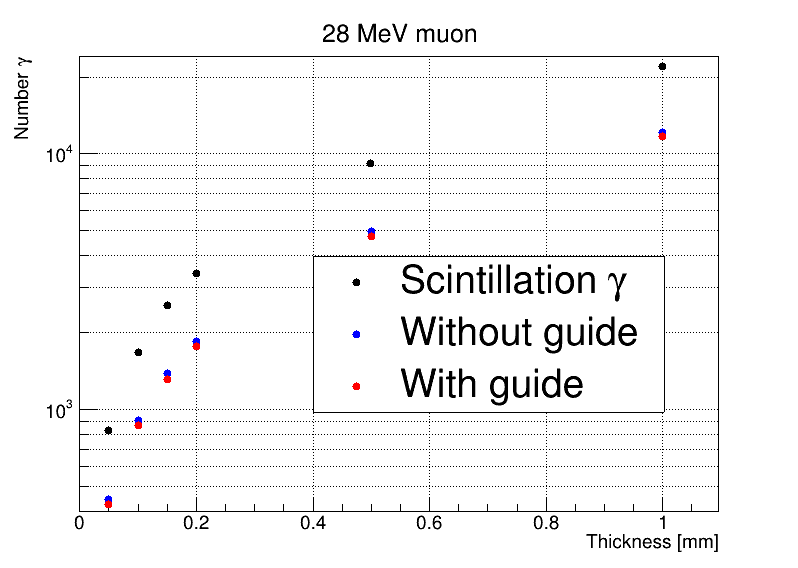
\includegraphics[height=5.5cm, keepaspectratio]{Figures/muEDM/Entrance/28mu_guide.png}\label{ffig:muEDM:entrance:guide:28mu}}
                \caption{asd}
                \label{fig:muEDM:entrance:guide}
            \end{figure}
    
            \begin{figure}   
                \centering
                \subfloat[A \SI{28}{MeV\per c} $\Am$ has $E_k \approx \SI{3.6}{MeV}$.]{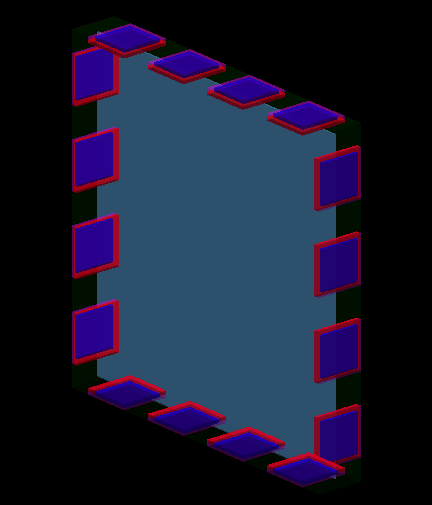
\includegraphics[height=5.5cm, keepaspectratio]{Figures/muEDM/Entrance/gate_noguide.png}}
                \hfill
                \subfloat[A \SI{128}{MeV\per c} $\Am$ has $E_k \approx \SI{60.3}{MeV}$.]{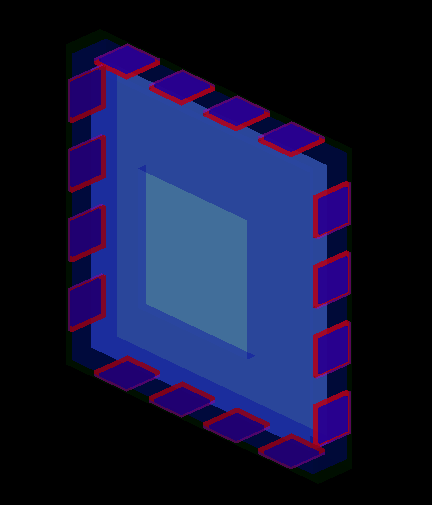
\includegraphics[height=5.5cm, keepaspectratio]{Figures/muEDM/Entrance/gate_guide.png}}
                \caption{asd}
                \label{fig:muEDM:entrance:guide:vis}
            \end{figure}
                
            \begin{figure}
                \centering
                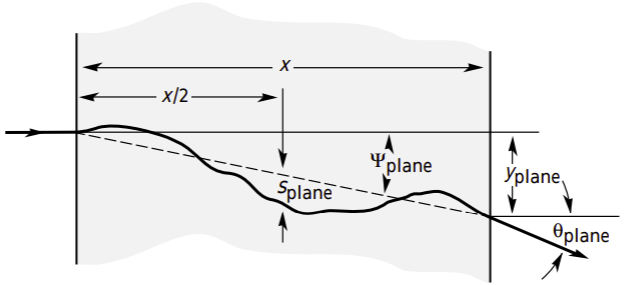
\includegraphics[width=0.6\textwidth]{Figures/muEDM/Entrance/multiple-scattering_pdg.png}\\
                \caption{}
                \label{fig:muEDM:entrance:pdgms}
            \end{figure}
    
            \begin{figure}   
                \centering
                \subfloat[ASD]{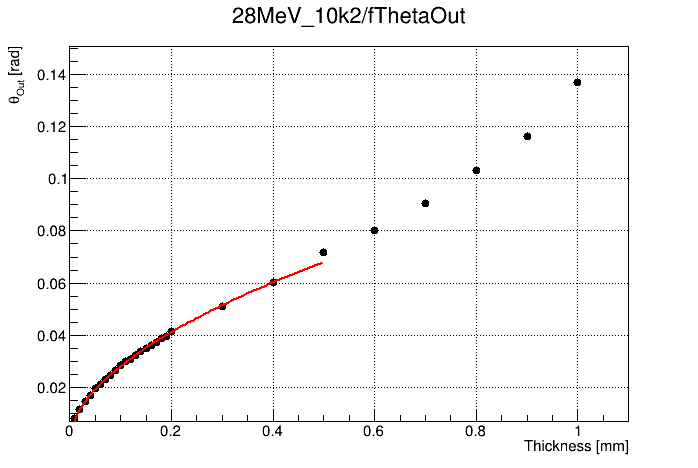
\includegraphics[height=5.5cm, keepaspectratio]{Figures/muEDM/Entrance/28mu_angleout_fit.png}\label{fig:muEDM:entrance:ms:28}}
                \hfill
                \subfloat[ASD]{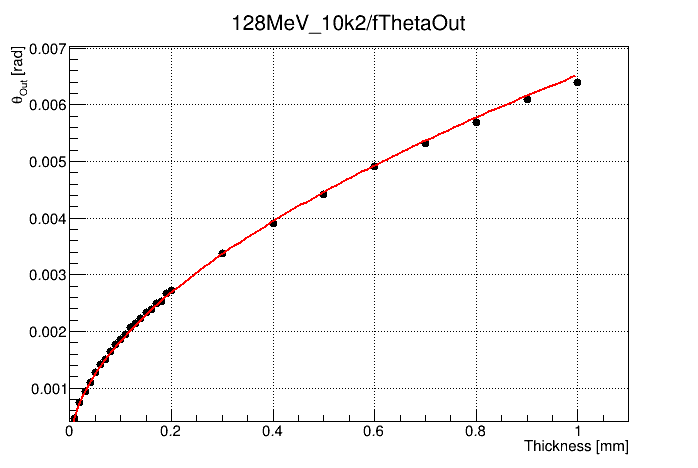
\includegraphics[height=5.5cm, keepaspectratio]{Figures/muEDM/Entrance/128mu_angleout_fit.png}\label{fig:muEDM:entrance:ms:128}}
                \caption{Average scattering angle in different thicknesses of \bc{400} scintillator for $\Am$ at \SI{28}{MeV\per c} and \SI{128}{MeV\per c}. From these plots was found $X_0 = \SI{54.33(12)}{g/cm^2}$.}
                \label{fig:muEDM:entrance:ms}
            \end{figure}
    
            \begin{figure}   
                \centering
                \subfloat[Possible readouts include all combinations of the different sides, like asking at least N sides, or $(s_1\land s_3)\lor(s_2\land s_4)$.]{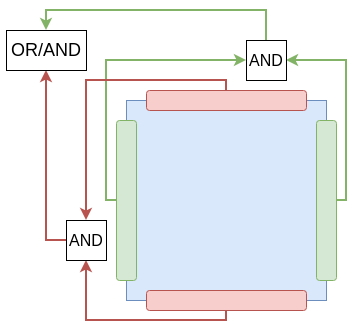
\includegraphics[height=5.5cm, keepaspectratio]{Figures/muEDM/Entrance/gate_multireadout.png}\label{ig:muEDM:entrance:gate:readout:guide}}
                \hfill
                \subfloat[Mounting a thin scintillator in a light guide can improve the photon collection. A `frame' shape prevents the incoming particle from interacting with additional material.]{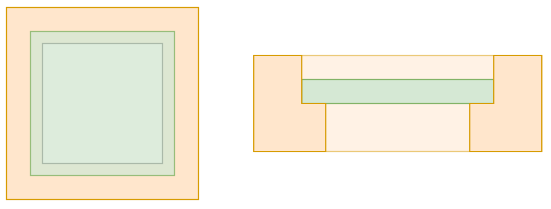
\includegraphics[height=3.5cm, keepaspectratio]{Figures/muEDM/Entrance/gate_waveguide.png}\label{ig:muEDM:entrance:gate:readout:multi}}
                \caption[muEDM: \textit{gate} scintillator readouts]{Two strategies to lower the threshold and improve the dark noise rejection: multiple readouts of a thin scintillator (a) and/or a light guide to improve the photon collection (b).}
                \label{ig:muEDM:entrance:gate:readout}
            \end{figure}


    \status{review}
    \subsection{Telescope and entrance detector}
        To study the entrance detector, a prototype was envisioned with a thin \textit{gate} scintillator read by multiple sides, a channel of 4 long scintillators creating a \textit{telescope}, and an additional scintillator as \textit{exit}.
        The development of such a system stems from the idea of having a way of vetoing the muons scattering at bigger angles while traversing the gate without requiring multiple detectors on the muon path.
        I started this simulation in \gf and it was later passed to the Shanghai colleagues, who further optimized and developed it using \textsc{musrSim}.
        The last step was to validate it with the data taken during the beamtime of 2022, discussed in Sec.~\ref{sec:muEDM:beamtime2022}.
        Although quite an interesting system, the collaboration decided not to implement it in the muEDM injection, deciding instead to rely on a Time Of Flight (TOF) measurement, which was tested in 2023 and sicussed in Sec.~\ref{sec:muEDM:beamtime2023}.
        \begin{figure}   
            \centering
            \subfloat[Front view of the detector system. \\The \textit{gate} is big enough to cover the aperture of the \textit{telescope}.]{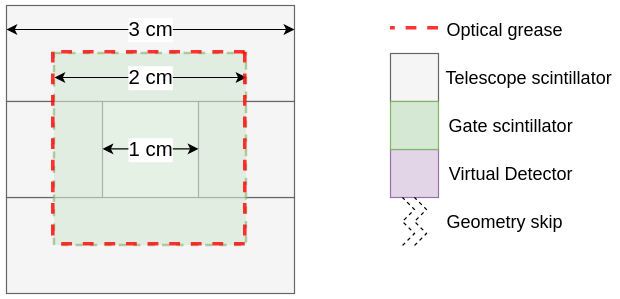
\includegraphics[height=4.5cm, keepaspectratio]{Figures/muEDM/Entrance/gate_geometry.png}\label{fig:muEDM:entrance:ms:28}}
            \hfill
            \subfloat[Side view of the syste. Additional VD used in the simulation for debugging are also shown.]{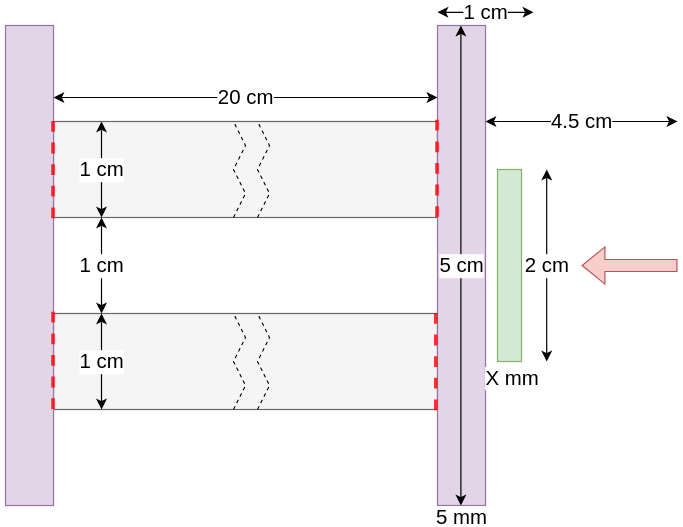
\includegraphics[height=5.5cm, keepaspectratio]{Figures/muEDM/Entrance/entrance_geometry.png}\label{fig:muEDM:entrance:ms:128}}
            \caption[muEDM: sketch if the \textit{telescope}]{Sketch of the first geometry for the \textit{gate} and \textit{telescope} detector for the 2022 muEDM beamtime. The aim was to test the thin \textit{gate} scintillator and the effect it has on the beam.}
            \label{fig:muEDM:entrance:sketches}
        \end{figure}
        
\status{review}
\section{Beamtime 2021}
\label{sec:muEDM:tim}
    This was the first muEDM beamtime I participated in. 
    I took an active part in the setup and measurement and I followed the analysis of the data collected. 
    This section relies on the Master Thesis of Tim Hume, part of the muEDM collaboration.
    This beamtime was designed to study the positron multiple scattering in different thin foils of the material expected to be viable solutions for the different parts of the experiment.
    On top of the material details, the aim was also to validate the scattering model used in the \gf simulations for further reference.
    The setup was quite simple: a telescope of five silicon pixel sensors,  three upstream and two downstream.

    \status{review}
    \subsection{Description of the multiple scattering}
        \paragraph{Highland}
        The Highland formula for multiple scattering is a parameterization for the width of the multiple scattering distribution.
        For a particle of charge $z$, momentum $p$ traversing a thickness of $x$ of a material with radiation length $X_0$, the RMS of the gaussian distribution is estimated as:
        \begin{equation}
        \label{eq:highland}
        \theta_0 = \frac{\SI{13.6}{MeV}}{\beta p c} z \sqrt{\frac{x}{X_0}} \left(1 + 0.038 \ln( \frac{x z^2}{X_0 \beta^2}) \right)
        \end{equation}
        Often, in the context of high particle physics, the projection on the directions orthogonal to the momentum are considered:
        \begin{equation}
        P(\theta_{x,y}) = \frac{1}{{\theta_0 \sqrt{2\pi}}} \exp\left(-\frac{\theta_{x,y}^2}{2\theta_0^2}\right)
        \end{equation}

        \paragraph{\gf}
        The default parameterization of the multiple scattering in \gf is the Urb\'{a}n. 
        This is based on a different description of the process, required because the evaluation is done at each step of the simulation, meaning \textit{within} the volume.
        This model describes the angular distribution of multiple scattering and samples it every interaction.
        The probability density of the angular distribution is usually indicated with $g(u)$ where $u = \cos \theta$ and the form is the following:
        \begin{equation}
            g(u) = \alpha +
            \begin{cases}
                \beta \exp(\gamma u) &\text{for } u_0 \le u \le 1 \\
                \delta (1-u)^\epsilon &\text{for } -1 \le u < u_0
            \end{cases}
        \end{equation}
        The parameter $u_0$ is the one used to transition between the central Gaussian-like distribution and the Rutherford-like tails at larger angles.\\

        \noindent
        For the Highland formula, the PDG reports an accuracy of $\sim 10\%$ in the range $\num{e-3}<x/X_0<\num{e2}$ \cite{PDG}, meaning it is less reliable for thin targets for which $x/X_0 \sim \mathcal{O}(\num{e-4})$.
        On the other hand, while \gf results have been widely tested against experimental measurements, there is a lack of data to compare in the ranges we are interested in.

    \status{review}
    \subsection{Data taking}
        The idea behind the data taking is quite simple: a study on the multiple scattering can be performed using a beam telescope, such as the one sketched in Fig~\ref{fig:muEDM:bt2021:telescope}, in which the two sides of the telescope are used to track the in/out-coming particles. 
        The delicate point is to carefully take into account the scattering of the particles in the telescope itself. 
        It is then needed to collect data without the sample to apply a deconvolution of the telescope response.
        The downstream part of the detector is not symmetrical to the upstream because only five sensors had the necessary performance. This made the tracking task more challenging, leading to wider distributions.
        The beamline used is the $\pi E1$, which provides $\uppi^\pm,\upmu^\pm,e^\pm$ in a momentum range $\SI{100}{MeV}\divisionsymbol\SI{500}{MeV}$.
        Clearly, a good understanding of the beam is key in both data-taking and analysis. 
        An example is the study of the beam changing the degrader's thickness, shown in Fig.~\ref{fig:muEDM:bt2021:TOF}.
        For brevity, the description of the electronics and DAQ system will be skipped. 

        \paragraph{Silicon Pixel Sensors}
        The sensors used are the last iteration of the sensors of the \textit{mu3e} experiment, the MuPix10. 
        These are High Voltage Monolithic Active Pixel Sensors (HV-MAPS) with $250\times256$ pixels of dimensions \SI{80}{\micro m}$\times$\SI{80}{\micro m}. 
        The sensor itself is on a PCB used for delivering the required voltages.
        A second, larger, PCB is set below the first and is responsible for reading and transmitting the data to FPGA.
        These sensors have been developed to achieve excellent position and time resolutions (\SI{100}{\micro m} and \SI{20}{ns}) with efficiency of $\varepsilon \approx 0.99$. 
        The thickness of these sensors is \SI{50}{\micro m} but this was the case for just the detector positioned after the samples. 
        The others were \SI{100}{\micro m}, important to be considered during the analysis.
        The whole apparatus is shown in Fig.~\ref{fig:muEDM:bt2021:setup:telescope} while a singular MuPix10 is shown in Fig.~\ref{fig:muEDM:bt2021:setup:MuPix10}.
        
        \begin{figure}
            \centering
            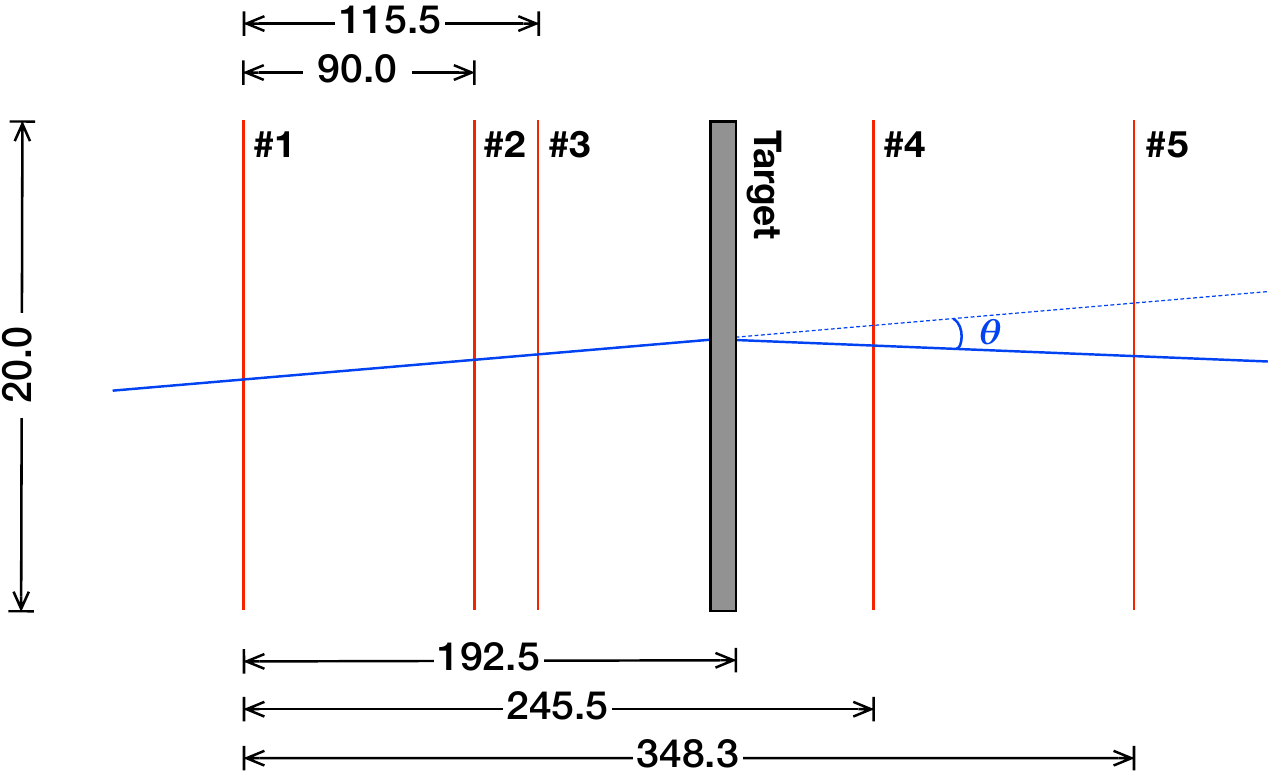
\includegraphics[width=0.6\textwidth]{Figures/muEDM_Dec2021/Positions_Telescope.png}\\
            \caption{Sketch of the telescope of Silicon Pixel Sensors used to study the multiple scattering in different materials.
            The samples are held in the position of the 'target'. 
            In this sketch, the beam is coming from the left side.}
            \label{fig:muEDM:bt2021:telescope}
        \end{figure}

        \begin{figure}   
            \centering
            \subfloat[Picture of the setup for the beamtime of 2021. On the right, the scintillator was used as an external trigger, on the left, beam exit window.]{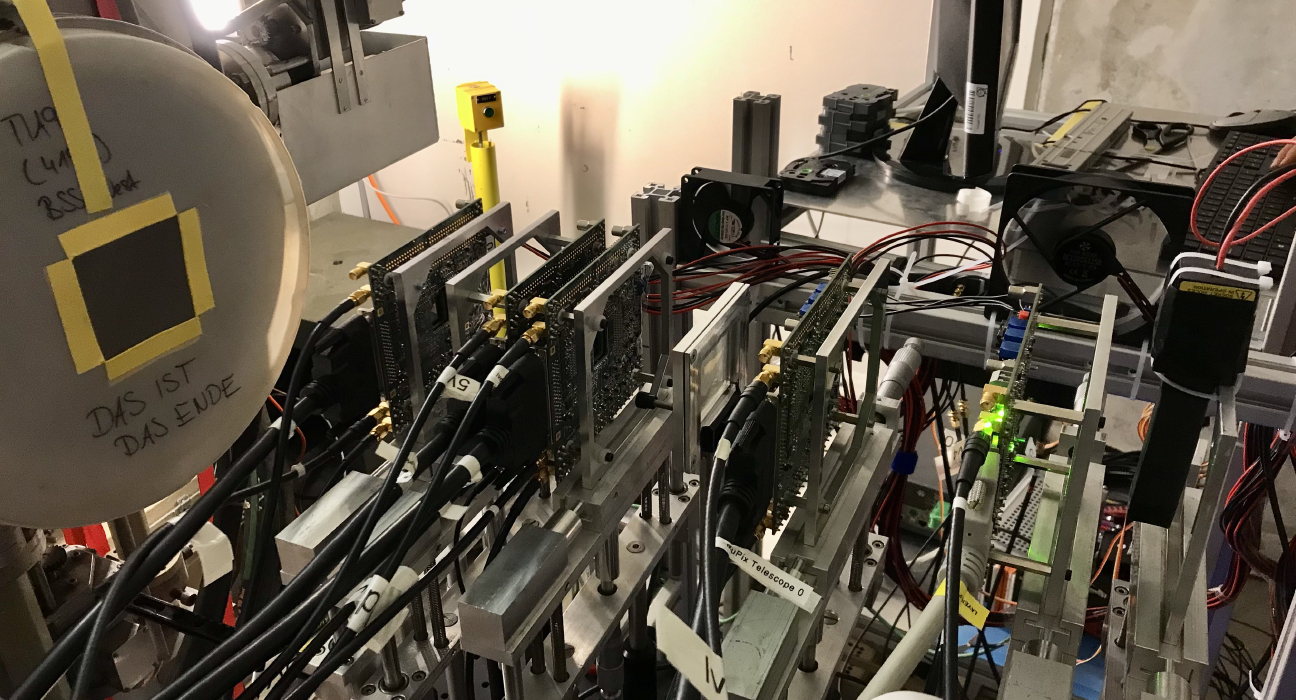
\includegraphics[height=5.5cm, keepaspectratio]{Figures/muEDM_Dec2021/Telescope_Picture.png}\label{fig:muEDM:bt2021:setup:telescope}}
            \hfill
            \subfloat[Picture of one of the MuPix10 mounted on the two PCBs.]{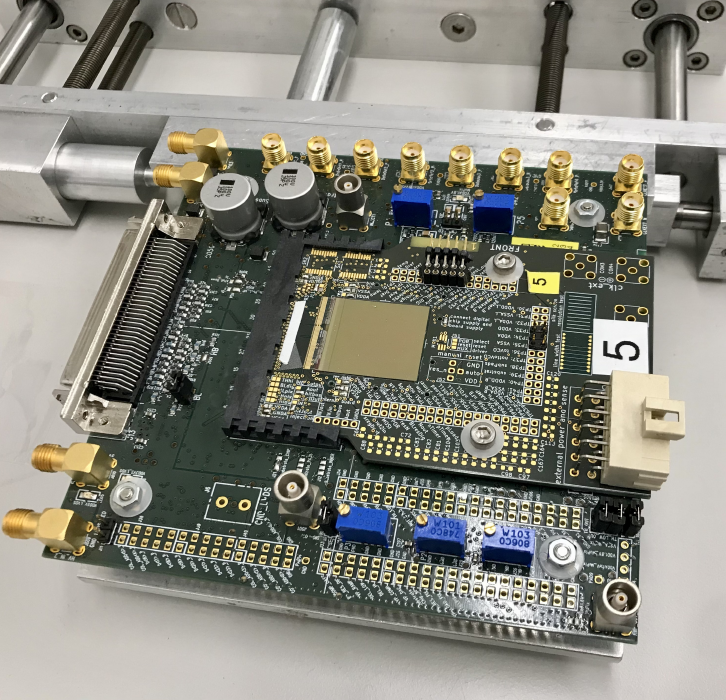
\includegraphics[height=5.5cm, keepaspectratio]{Figures/muEDM_Dec2021/MuPix10_Picture.png}\label{fig:muEDM:bt2021:setup:MuPix10}}
            \caption{Picture of the setup and one of the MuPix10 (grey-colored square) mounted on the PCBs.}
            \label{fig:muEDM:bt2021:setup}
        \end{figure}

        \begin{figure}
            \centering
            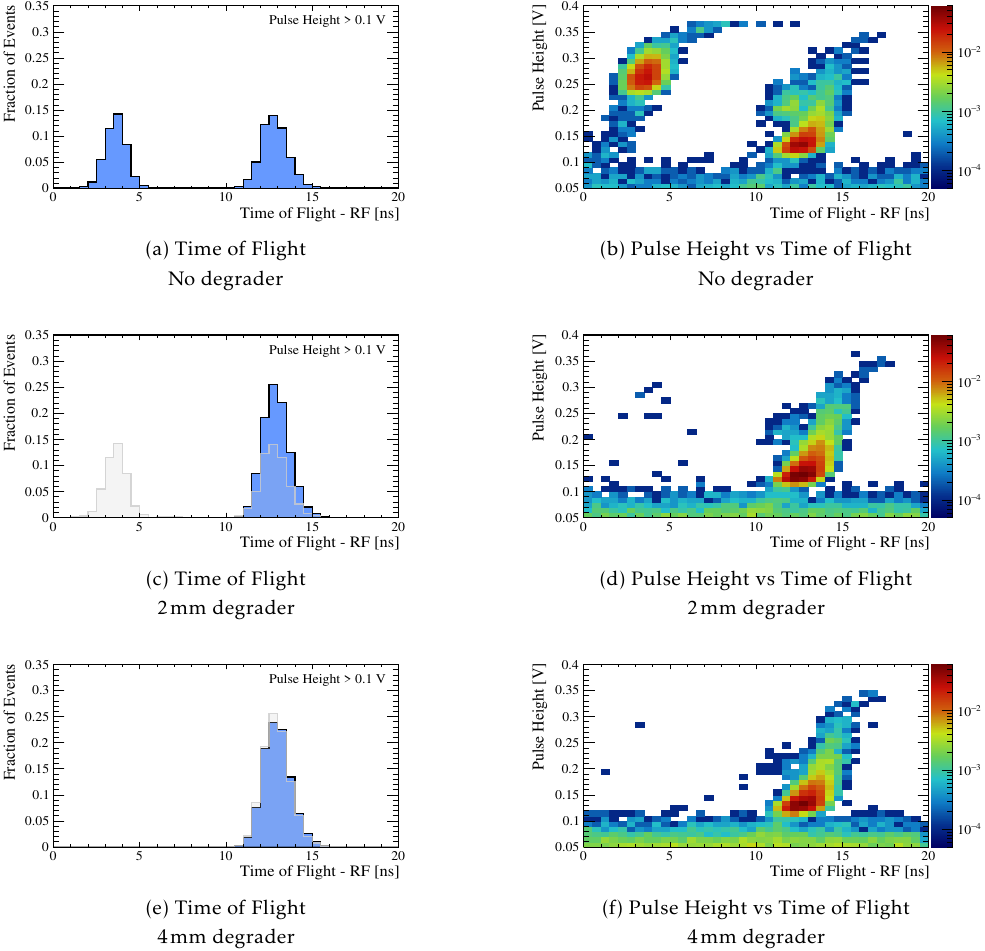
\includegraphics[width=0.9\textwidth]{Figures/muEDM_Dec2021/muEDM_beamtime2021_TOF.png}
            \caption{Timing and the 2D plot for time and pulse height for \SI{120}{MeV/c} particles. The three rows show what happens when inserting degraders of different thicknesses.
            With no degrader, the $\uppi$ peak is visible at lower TOF.
            When increasing the thickness, the contributions of $\uppi$ and $\upmu$ decrease.
            It is important to note that the $e$ and $\upmu$ distribution overlap.
            In gray the distribution of the previous plot to make a comparison.}
            \label{fig:muEDM:bt2021:TOF}
        \end{figure}

    \status{review}
    \subsection{Data analysis}
        \paragraph{Track selection}
        Initial angular distributions obtained were broad due to noise in downstream sensors, making it difficult to distinguish noise from true hits. 
        To address this, a filtering process was developed to select the track candidate with the least spatial separation between the intersections of upstream and downstream tracks on the plane of the sample.
        The expected angular distribution for particles passing through a material at normal incidence should be spatially symmetric and independent of chosen projection axes. 
        Any deviation from this symmetry could indicate experimental, data processing, or analysis errors. 
        To mitigate the effects the idea was to combine distributions from multiple axes.
        In the initial distributions, the broad background can be attributed to false tracks generated by noise, poor fits, and some contribution of events with large angles of scattering in the telescope itself. 
        This background was suppressed by enforcing a distance of \SI{1}{mm} between the points at which the upstream and downstream tracks intersect the plane of the sample.        
        Distributions before and after applying this filter are shown in black and red in Fig.~\ref{fig:muEDM:bt2021:distributions}
        This distribution was then corrected for the geometric acceptance of the telescope.
        \begin{figure}
            \centering
            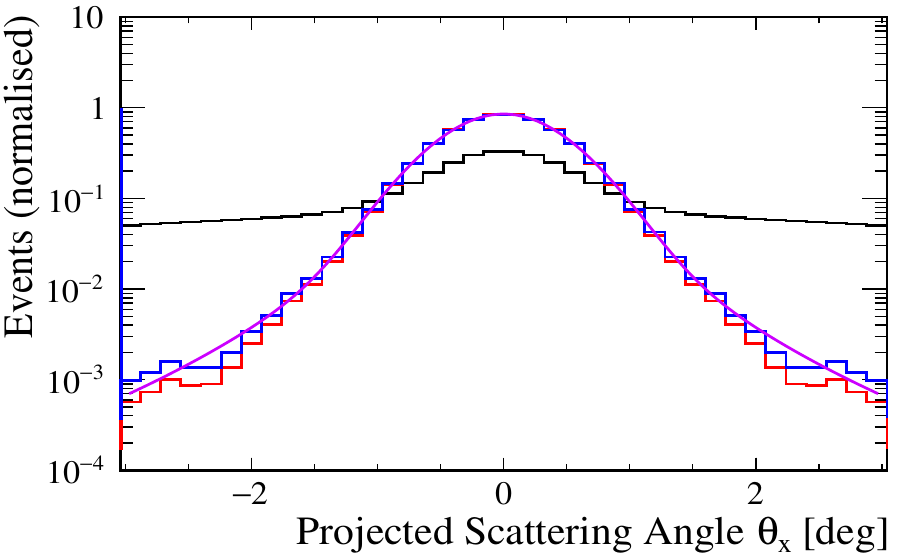
\includegraphics[width=0.8\textwidth]{Figures/muEDM_Dec2021/distributions.png}
            \caption{The angular distributions show: the full distribution (black), the distribution after cuts in the distance at the sample's plane (red), the distribution after acceptance correction (blue), and the fitted function for telescope characterization (violet).}
            \label{fig:muEDM:bt2021:distributions}
        \end{figure}
        
        \paragraph{Acceptance}
        The correction for the geometrical acceptance of the telescope was essential to accurately determine the tails of the angular distribution.
        To estimate the acceptance, for each upstream track identified, scattering angles were randomly assigned and added to a histogram, distinguishing instances within the acceptance of the most downstream sensor. 
        The ratio of histograms yielded the average acceptance as a function of projected scattering angles. 
        The acceptance correction was applied on a per-event basis, adjusting the scattering angles based on the acceptance value. 
        An example of such correction is shown in blue in Fig.~\ref{fig:muEDM:bt2021:distributions}
        
        \paragraph{Deconvolution}
        The method of track selection and acceptance correction was applied to both runs with and without the sample. 
        The distributions from these runs were then fitted.
        The process involved:
        \begin{outline}
            \1 Characterizing the telescope's response without the sample using a weighted sum of a Gaussian distribution and a Student's t distribution
            \1 Convolving the response function with the sample's angular distribution, assumed to follow a single Student's t distribution
            \1 using the negative log-likelihood to determine the best-fit parameters for describing the measured distribution with the sample
        \end{outline}
    
    \status{review}
    \subsection{Model evaluation and conclusions}
        This first beamtime aimed at testing the agreement between the Highland formula and the \gf Urb\'{a}n model for the multiple scattering in thin materials.
        The analysis of the data collected is still not finalized, but a rough agreement between data and models can be seen in Fig.~\ref{fig:muEDM:bt2021:results}.
        Some improvements could be added to the analysis and/or to the simulation of the experimental setup, so updated results are expected in the following months.
        
    \begin{figure}   
            \centering
            \subfloat[Pokalon (orange), \SI{17}{\micro m} Graphite (blue), \SI{50}{\micro m} Graphite (violet), Silicon (red); circular markers for data at \SI{70}{MeV}, squared at \SI{90}{MeV}; error bars are the statistical and the shaded the total uncertainties.]{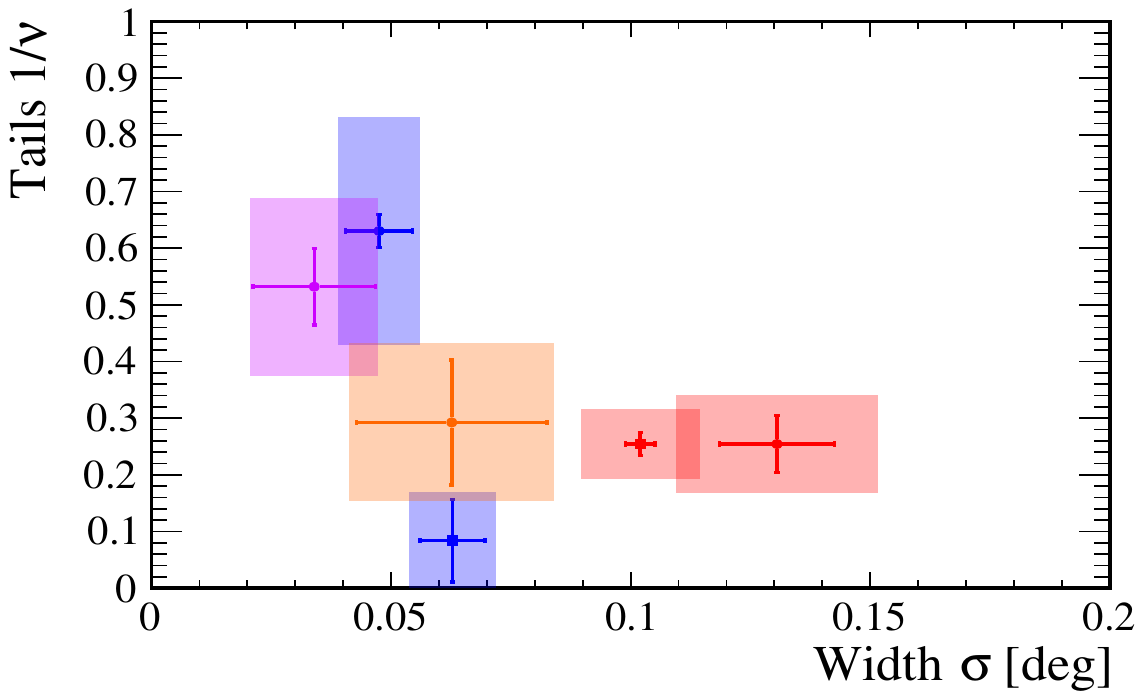
\includegraphics[width=0.48\textwidth, keepaspectratio]{Figures/muEDM_Dec2021/ms_fits.png}\label{fig:muEDM:bt2021:results:analysis}}
            \hfill
            \subfloat[Same color/shape coding as Fig.~\ref{fig:muEDM:bt2021:results:analysis} and the predictions of the Highland formula are shown by lines of width representing the uncertainty in thickness.]{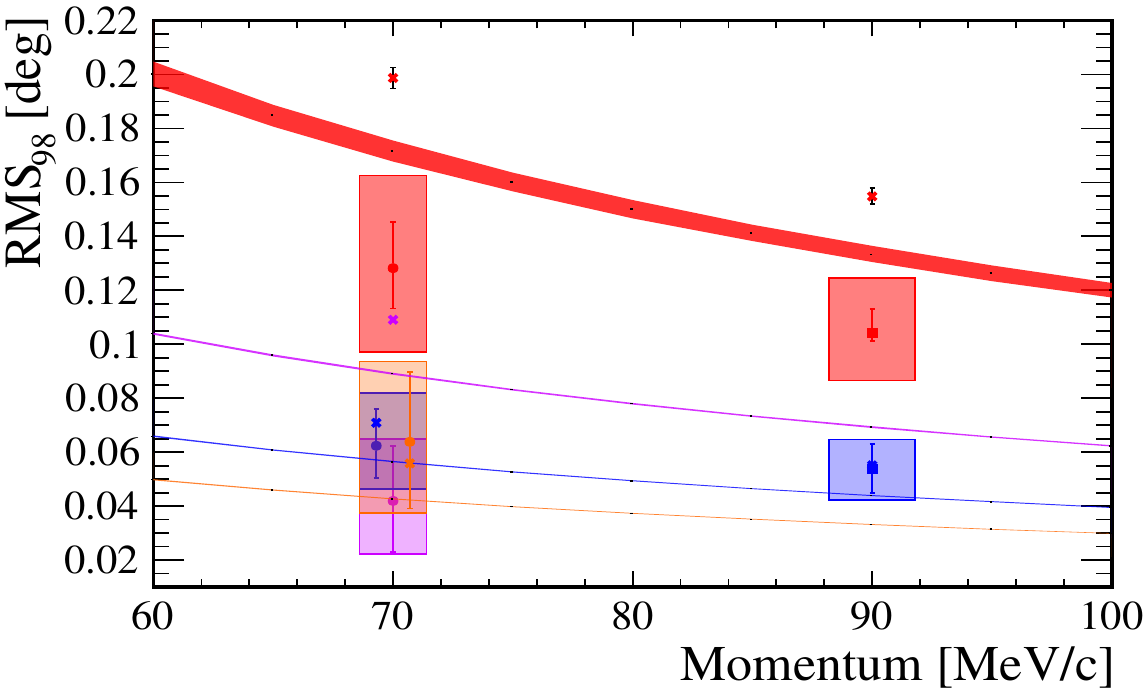
\includegraphics[width=0.48\textwidth, keepaspectratio]{Figures/muEDM_Dec2021/gf-highland_evaluation.png}\label{fig:muEDM:bt2021:results:models}}
            \caption{Results of the analysis of the different samples and confronted with predictions using the Highland formula and \gf. The details are not easy to read but the 'bring-home' message is that the results are somewhat in agreement and some improvement are planned on the analysis.}
            \label{fig:muEDM:bt2021:results}
        \end{figure}

\status{review}
\section{Beamtime 2022: Telescope and entrance detector}
\label{sec:muEDM:beamtime2022}
    This second beamtime\footnote{Not counting the one for the \tpc + \grid of Sec.~\ref{sec:muEDM:gridpix:beamtime}.} happened in November 2022.
    The aims were:
    \begin{outline}
        \1 Test of entrance scintillator with the additional `telescope'
        \1 parasitic measurements for the \tpc+ \grid
    \end{outline}
    This time I, together with Prof. Angela Papa and David St\"{a}ger (a master student from ETH) participated actively in the development of the setup. 
    In particular, we took care of the entrance scintillator, auxiliary detectors, the electronic, vacuum system, and one version of the telescope. 
    To test different reading options a second telescope was developed by the Shanghai part of the collaboration and they also helped develop the mechanical structure.

    \status{review}
    \subsection{Construction}
        \paragraph{Scintillators}
        The thin scintillators used during this beamtime had already been tested for previous purposes. 
        We had \SI{100}{\micro m} and \SI{200}{\micro m} to be used as entrance and exit from the telescope.
        These were already mounted on PCB boards with multiple SiPMs as readouts. The SiPMs were read all together so the sum of the signals was the only information available.
        An example of this setup is shown in Fig.~\ref{fig:muEDM:thin_scintillators}.
        On the other side, the long scintillators which compose the telescope were not already available.
        Two versions were built in parallel.
        \begin{outline}
            \1 The "Shanghai's version" was made of $200\times 20\times\SI{10}{mm}$ scintillators read on one side.
            \1 The "Pisa's version" was made of $200\times 25\times\SI{5}{mm}$ scintillators read on both sides.
        \end{outline}
        Two versions were built to study how much the longitudinal information of the hits on the telescope would benefit the study of the overall system.
        I worked on the soldering of the SiPMs on the PCB boards for the readout (3 per side).
        Then I glued the scintillators using \textit{optical cement}.
        The gluing to the PCB is shown in Fig.~\ref{fig:muEDM:bt2021:setup:gluing}.
        Gluing the scintillators this way, we knew small gaps between them after mounting the telescope were unavoidable. 
        This was actually to confront it with the Shanghai telescope\footnote{Being my first gluing I used too much optical cement, which further increased the gap between crystals.}, for which the cross-talk between different crystals was expected.

        \begin{figure}
            \centering
            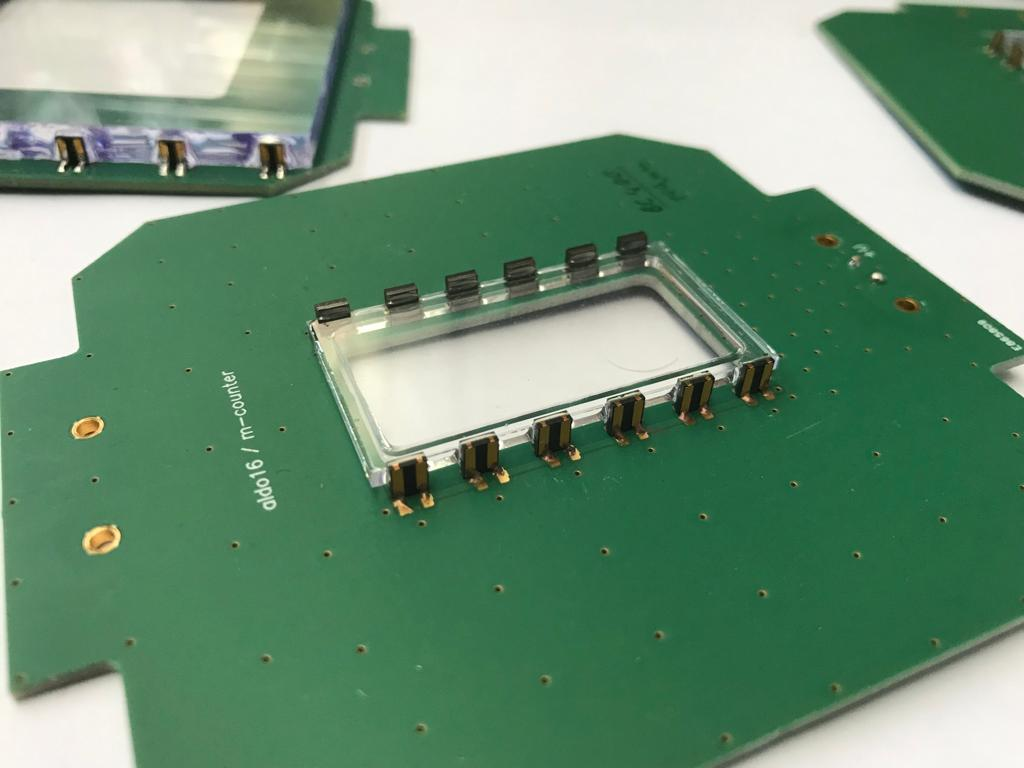
\includegraphics[width = 0.8\textwidth]{Figures/muEDM/thin_scintillators.jpg}
            \caption[muEDM: Thin scintillators for the beamtimes.]{Picture of different scintillators mounted on PCBs and read by multiple SiPMs. The signals of the SiPMs are summed and different thicknesses were already available at the time of the 2021 beam time.}
            \label{fig:muEDM:thin_scintillators}
        \end{figure}

        \paragraph{Electronics}
        The First challenge was to bring the necessary power to the detectors and bring the readout out of the vacuum chamber.
        The choice was to use a WaveDream board as a DAQ unit for this beamtime.
        We custom-made the necessary feed-throughs, gluing with \stycast PCB boards through two blind flanges.
        The connectors were then soldered to the PCB, creating the feed-throughs shown in Fig.~\ref{fig:muEDM:bt2021:setup:feedthrough}.
        
        \paragraph{Final setup}
        Combining the thin scintillators as \textit{gate} and \textit{exit} with the telescope and the needed feed-throughs we get the complete setup shown in Fig.~\ref{fig:muEDM:bt2021:telescope:front}.
        The las additions were a \textit{veto} scintillator ($100\times 100\times\SI{5}{mm}$ with a circular \SI{10}{mm} hole) to optimize the particle selection and a tube to contain the whole thing.
        For this last item, to allow the feed-throughs to be on the side of the setup, we used a "T" beampipe piece, shown in Fig.~\ref{fig:muEDM:bt2021:telescope:built}.
        
        \begin{figure}   
            \centering
            \subfloat[Custom feed-throughs: PCB board, with soldered connectors, sealed with Stycast in a blind flange.]{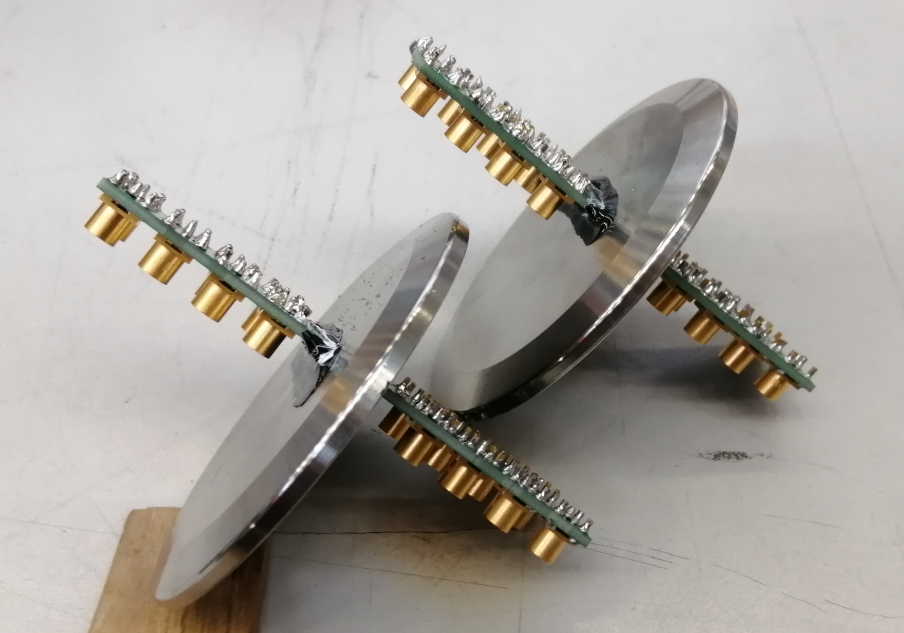
\includegraphics[width=0.49\textwidth, keepaspectratio]{Figures/muEDM_Nov2022/feedthrough.png}\label{fig:muEDM:bt2021:setup:feedthrough}}
            \hfill
            \subfloat[A small PCB board with 3 SiPMs and one connector attached with optical cement to one of the scintillators.]{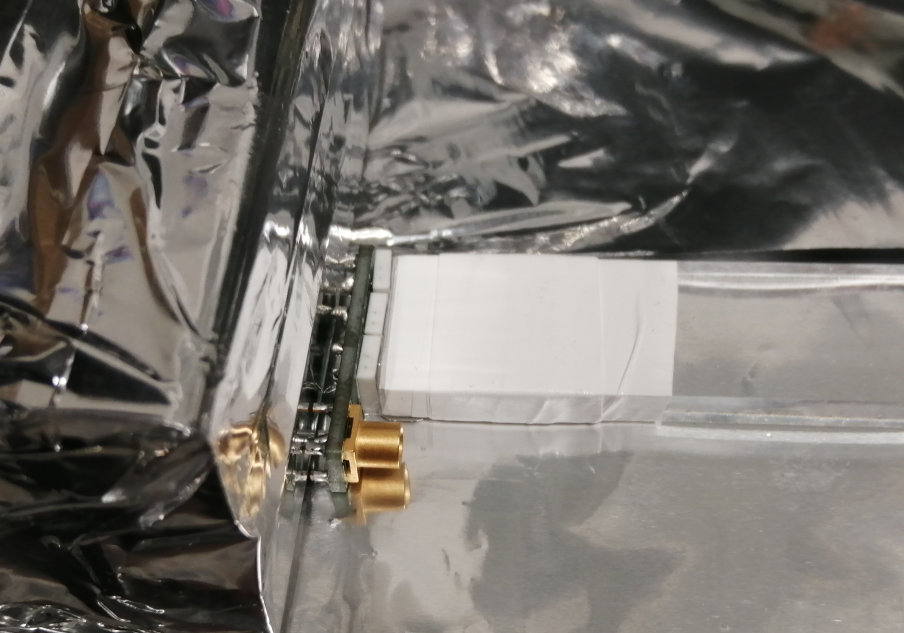
\includegraphics[width=0.49\textwidth, keepaspectratio]{Figures/muEDM_Nov2022/SIPMgluing.png}\label{fig:muEDM:bt2021:setup:gluing}}
            \caption[muEDM 2022: entrance preparations]{Part of the preparation needed for the beamtime was to develop the detectors, as well as the vacuum in which the measurement would have taken place.}
            \label{fig:muEDM:bt2021:setup}
        \end{figure}
        
        \begin{figure}   
            \centering
            \subfloat[Assembly of the \textit{telescope} with \textit{entrance} and \textit{veto}.]{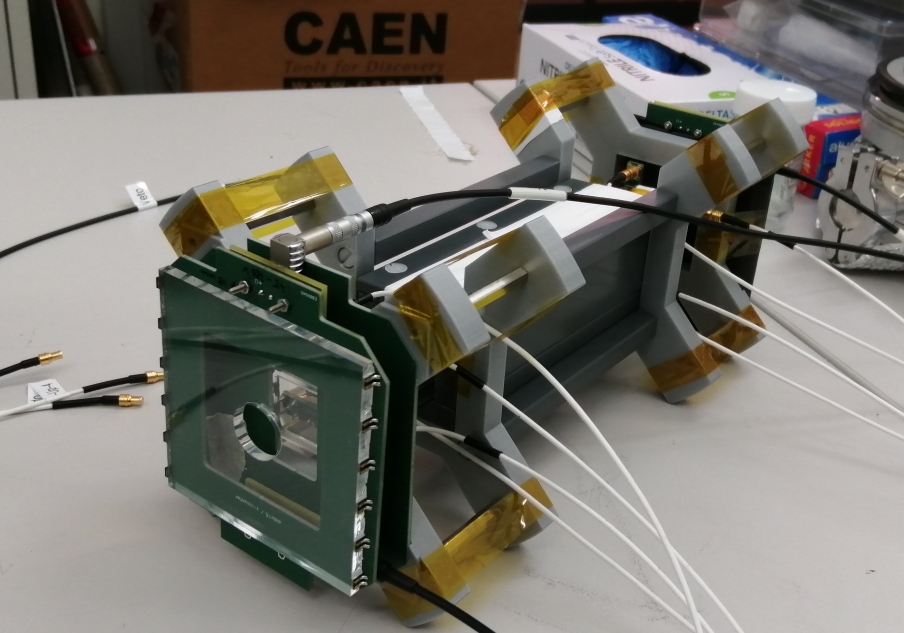
\includegraphics[width=0.49\textwidth, keepaspectratio]{Figures/muEDM_Nov2022/telescope_front.png}\label{fig:muEDM:bt2021:telescope:front}}
            \hfill
            \subfloat[``T'' beamline piece used as vacuum chamber.]{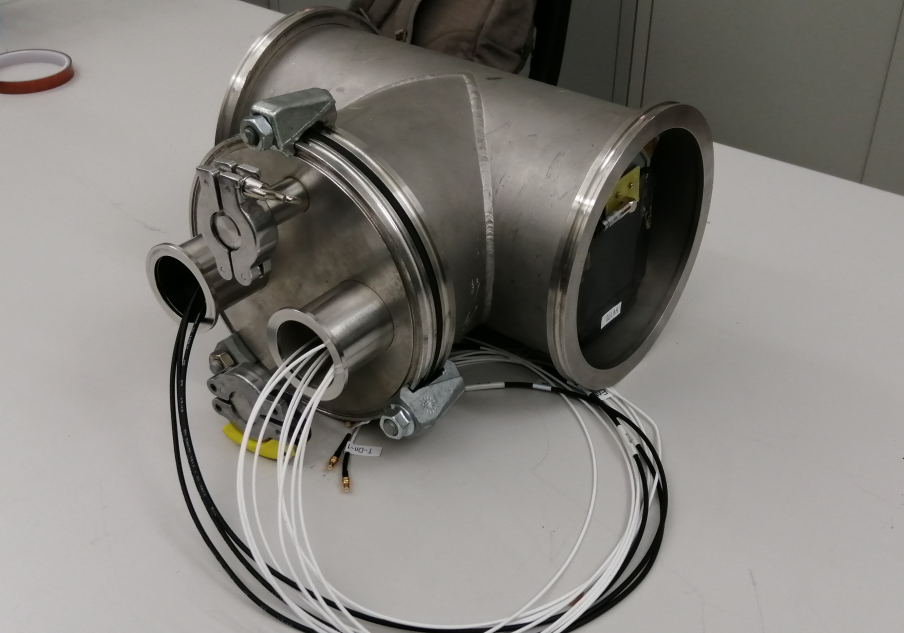
\includegraphics[width=0.49\textwidth, keepaspectratio]{Figures/muEDM_Nov2022/telescope_built.png}\label{fig:muEDM:bt2021:telescope:built}}
            \caption[muEDM 2022: entrance setup]{The \textit{entrance} scintillator, the \textit{telescope}, and the \textit{veto} were assembled in a rigid structure. A ``T'' beamline piece was used to put the detector in the beamline. The lateral flange was adapted for the feedthroughs while, on the back, a \mylar widow was mounted to allow further measurements of the beam.}
            \label{fig:muEDM:bt2021:telescope}
        \end{figure}

        \paragraph{Additional items}
        After the system just described, two more items were added:
        \begin{outline}
            \1 SIMON/PIL: Beam monitors were used to characterize the beam.
            \1 \tpc+ \grid: Used parasitically to gather some missing details, which were merged to the data from 2021 beam-time in the publication already mentioned (see Sec.~\ref{sec:muEDM:gridpix:beamtime}) \cite{muEDM:PSI:GridPix}.
        \end{outline}

    \status{review}
    \subsection{Data taking}
        The whole beamtime was roughly two weeks. 
        The first days were dedicated to the beam tuning and measurements.
        Two settings were defined to have the beam focused on the gate or the exit scintillator. 
        These two setups allowed us to study different aspects of the prototype, which will be discussed in the following section.
        For each channel, supply and threshold were decided by measuring the rate of triggers with/without a \ce{Sr90} source. 
        A picture of the end of the beamline and the setup is in Fig.~\ref{fig:muEDM:bt2022:setup:beam} while in  Fig.~\ref{fig:muEDM:bt2022:setup:window} the end Mylar window before being covered with Teflon to make it light tight.
        The DAQ of choice was a standalone WaveDREAM.
        Different trigger configurations were used to study the different aspects of the setup. 
        A `typical' trigger window of the DAQ system is shown in Fig.~\ref{fig:muEDM:bt2022:triggers}.
        In this, a dot means that channel is required while a cross means it is used as a veto\footnote{We later found out this feature was bugged and we had to manually set up a veto system using NIM modules.}.
        The system has 16 channels and 18 triggers.
        
        \begin{figure}
            \centering
            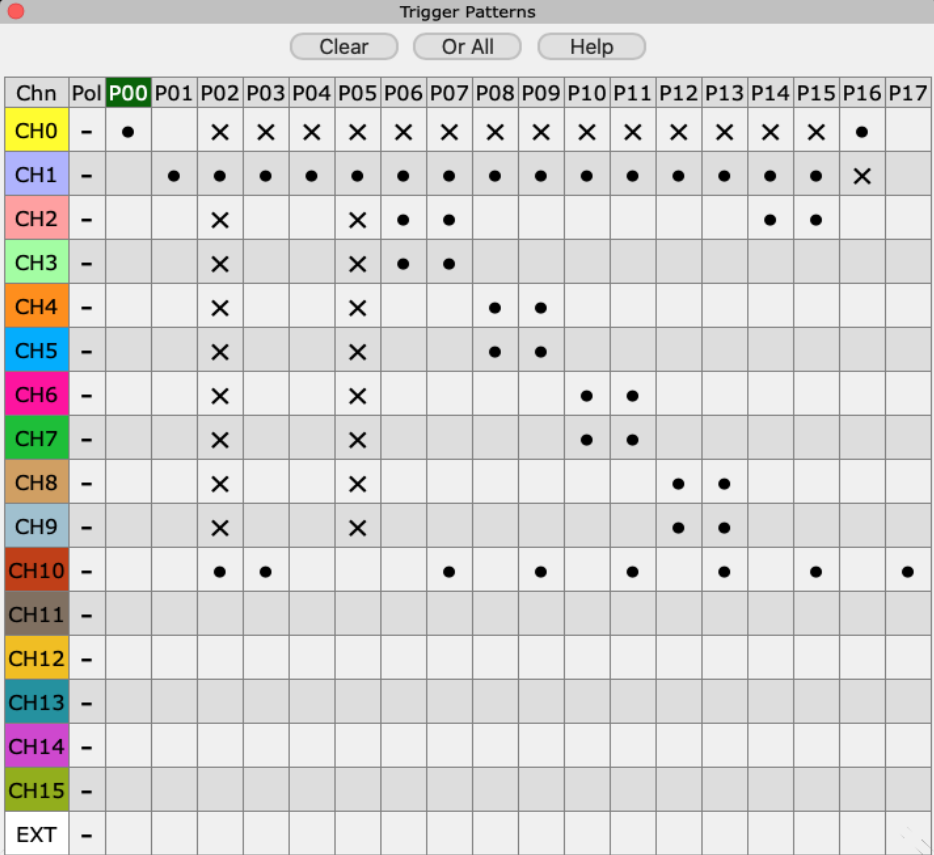
\includegraphics[width = 0.8\textwidth]{Figures/muEDM_Nov2022/muEDM2022_triggers.png}
            \caption[muEDM:2022 triggers]{WaveDREAM interface to set the triggers. A dot is a required channel while a cross is used as veto. Some examples are: P00 - veto only; P01 - gate only; P03 - !veto \& gate \& exit.}
            \label{fig:muEDM:bt2022:triggers}
        \end{figure}
        
        \begin{figure}   
            \centering
            \subfloat[The setup mounted at the end of the beamline.]{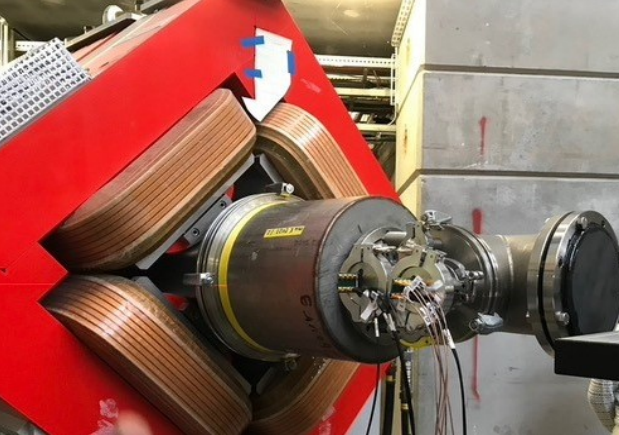
\includegraphics[width=0.45\textwidth, keepaspectratio]{Figures/muEDM_Nov2022/muEDM2022_beamtuning.png}\label{fig:muEDM:bt2022:setup:beam}}
            \hfill
            \subfloat[The view of the detectors from the Mylar window before making it light-tight.]{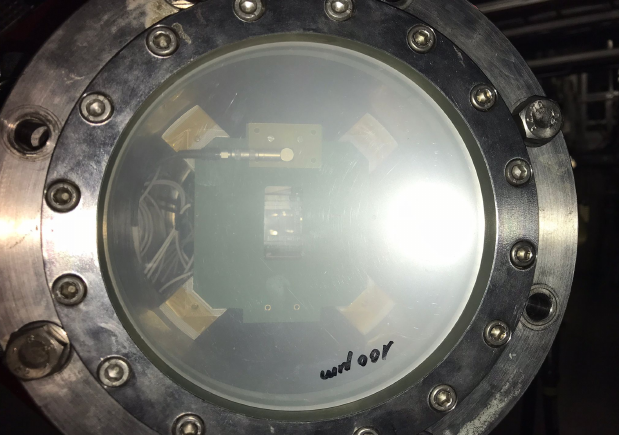
\includegraphics[width=0.45\textwidth, keepaspectratio]{Figures/muEDM_Nov2022/muEDM2022_window.png}\label{fig:muEDM:bt2022:setup:window}}            
            \caption[muEDM:2022 installation]{Pictures of the system after the installation along the beamline.}
            \label{fig:muEDM:bt2022:blobs}
        \end{figure}
        
    \status{review}
    \subsection{Data analysis}
        The data collected were analyzed in parallel to study the behavior of the gate and the telescope. 
        The first will be part of the muEDM experiment, the second was developed to test such a system.

        \subsubsection{Gate}
            The main aim is to evaluate the current efficiency of the gate and evaluate if/how to improve it, to have a reliable trigger for the magnetic kicker.
            For this measurement, the events were triggered with the exit scintillator, ensuring the muon had to pass through the gate.
            Changing offline the charge requirement on the gate, the efficiency vs threshold can be evaluated.
            Taking into consideration also the time difference between the gate and exit we can construct a 'side-band' to correct for accidental coincidences.
            The plot resulting is in Fig.~\ref{fig:muEDM:bt20212gate} and the results are summarized in table Tab.~\ref{tab:muEDM:bt2022:gate}.
            From these is clear a low threshold is required to achieve high efficiency in detecting \SI{28}{MeV/c}.
            Looking at the values obtained for the thermal noise for this detector (see Tab.~\ref{tab:muEDM:bt2022:gatenoise}), unfortunately, the readout implemented does not allow to reduction of the threshold without hitting the thermal noise.
            This was somewhat expected, and for this reason, the beamtime of 2023 (see Sec.~\ref{sec:muEDM:beamtime2023}) was planned to test a 4-way readout to require coincidences between channels.\\

            \begin{figure}
                \centering
                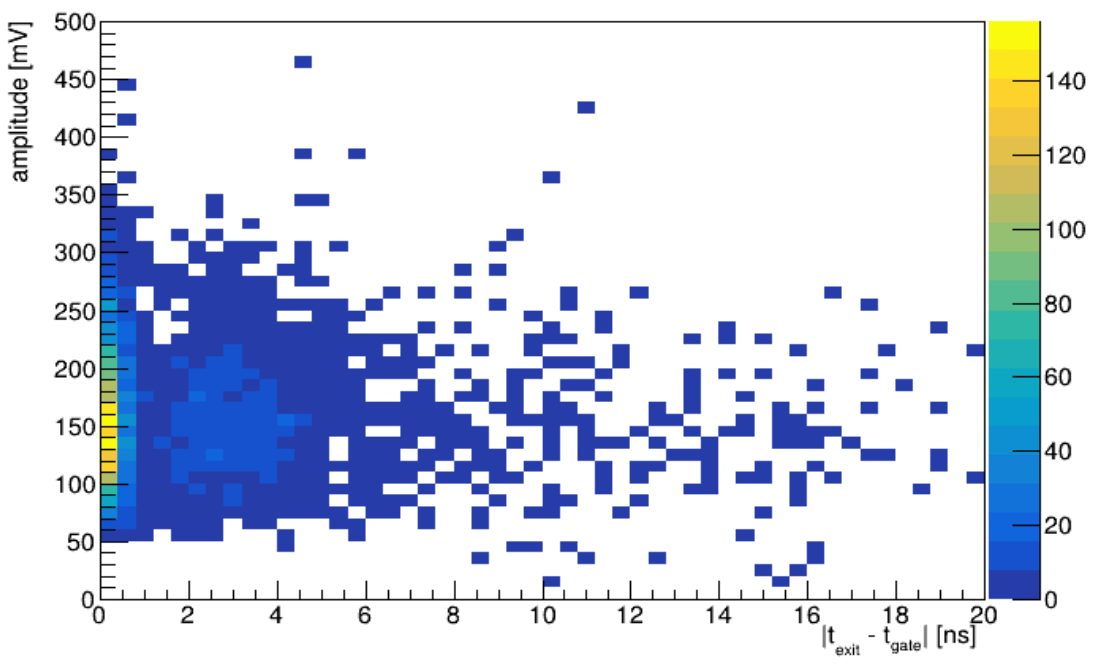
\includegraphics[width = 0.8\textwidth]{Figures/muEDM_Nov2022/gate_eff-time.png}
                \caption[muEDM:2022 gate efficiency]{Correlation plot for the amplitude of the signal in the gate and the TOF measured. If this plot is produced while triggering only on the exit, it can be used to evaluate the gate efficiency.}
                \label{fig:muEDM:bt20212gate}
            \end{figure}
            
            \begin{table}[ht]
              \begin{minipage}{0.55\textwidth}
                \centering
                \begin{tabular}{|c|c|c|c|c|c|c|}
                \hline
                & \multicolumn{3}{c|}{10 ns} & \multicolumn{3}{c|}{5 ns} \\
                \hline
                Thr. [mV] & $N_{coin}$ & $N^{acc}_{coin}$ & $\varepsilon$ [\%] & $N_{coin}$ & $N^{acc}_{coin}$ & $\varepsilon$ [\%] \\
                \hline
                -50 & 3798 & 130 & 91.7 & 3549 & 65 & 87.1 \\
                -100 & 3385 & 116 & 81.8 & 3169 & 58 & 77.8 \\
                -150 & 2067 & 64 & 50.1 & 1934 & 32 & 47.6 \\
                -200 & 820 & 30 & 19.8 & 768 & 15 & 18.8 \\
                -250 & 266 & 8 & 6.5 & 253 & 4 & 6.2 \\
                \hline
                \end{tabular}
                \captionof{table}[Efficiency for gate threshold]{Number of coincidences, accidentals, and efficiency as a function of the gate threshold.}
                \label{tab:muEDM:bt2022:gate}
              \end{minipage}\hfill
              \begin{minipage}{0.4\textwidth}
                \centering
                \begin{tabular}{|c|c|c|}
                \hline
                \thead{Thr.\\[0.1ex] [mV]} & \thead{\SI{100}{\micro\meter} gate \\ noise [kHz]} & \thead{\SI{200}{\micro\meter} exit \\ noise [kHz]} \\
                \hline
                -20 & 1435 $\pm$ 5 & 16,750 $\pm$ 50 \\
                -30 & 643 $\pm$ 2 & 8800 $\pm$ 50 \\
                -40 & 287 $\pm$ 1 & 4350 $\pm$ 50 \\
                -50 & 150 $\pm$ 1 & 2350 $\pm$ 50 \\
                -60 & 78 $\pm$ 0.5 & 1330 $\pm$ 20 \\
                -70 & 42 $\pm$ 0.5 & 745 $\pm$ 5 \\
                -80 & 23.7 $\pm$ 0.2 & 435 $\pm$ 5 \\
                -90 & 13.3 $\pm$ 0.3 & 250 $\pm$ 3 \\
                -100 & 7.2 $\pm$ 0.1 & 141 $\pm$ 2 \\
                -150 & 0.6 $\pm$ 0.02 & 11.5 $\pm$ 0.5 \\
                -200 & 0.04 $\pm$ 0.01 & 1.2 $\pm$ 0.05 \\
                -250 & $\approx$ 0.005 & 0.13 $\pm$ 0.02 \\
                -275 & $\approx$ 0.001 & 0.04 $\pm$ 0.01 \\
                -375 & $\approx$ 0 & $\approx$ 0.001 \\
                \hline
                \end{tabular}
                \captionof{table}{Thermal noise rates at different thresholds for gate/exit scintillators.}
                \label{tab:muEDM:bt2022:gatenoise}
              \end{minipage}
            \end{table}

            \noindent
            Another key aspect of the gate scintillator we wanted to study was the time resolution, a key parameter for the triggering of the magnetic pulser, and a TOF detector for the CW/CCW analysis discussed in the section on systematics (Sec.~\ref{sec:muEDM:systematics}).
            Evaluating the time difference between gate and exit we can evaluate the time of flight of the particles. 
            The spread of this measurement is the convolution of the momentum spread and the intrinsic resolution of the system made of the two scintillators: $\sigma_{TOF} = \sigma_{p} \oplus \sigma_{scint}$.
            Given gate and exit have different thicknesses, their contribution will be only approximated by $\sigma_{scint}\approx\sqrt{2}\sigma_{gate/exit}$.
            The result of the Gaussian fit on the TOF measurement is in Fig.~\ref{fig:muEDM:bt20212gate:resolution} and the resulting res9olution is $\sigma_{TOF} \approx \SI{241}{ps}$.
            Assuming a 3\% momentum spread, the resulting resolution of the detector is $\sigma_{scint}\approx 241 \ominus \SI{78}{ps} \approx \SI{228}{ps}$.
            From this we can make a rough estimate of $\sigma_{gate}\approx\SI{228}{ps}/\sqrt{2} \approx\SI{160}{ps}$.
            These results are completely satisfying.

            \begin{figure}
                \centering
                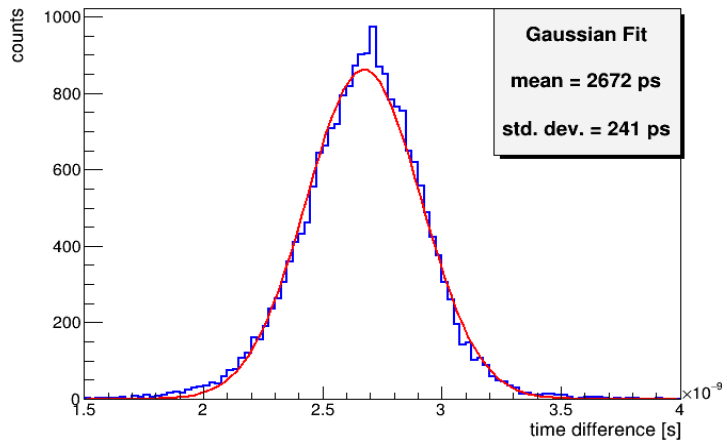
\includegraphics[width = 0.8\textwidth]{Figures/muEDM_Nov2022/gate_resolution.png}
                \caption[muEDM:2022 time resolution]{Measuring the TOF resolution, and assuming a momentum spread of 3\%, we can extract a combined resolution of gate and exit of $\sigma_{scint}\approx 241 \ominus \SI{78}{ps} \approx \SI{228}{ps}$. This result meets the requirements.}
                \label{fig:muEDM:bt20212gate:resolution}
            \end{figure}

        \subsubsection{Telescope}
            \noindent
            Naively one might expect that either the muon undergoes a small scatter in the gate and gets to the exit scintillator, or is scattered at a bigger angle and is stopped in one of the scintillators creating the telescope.
            In reality, the position of the beam focus and the trigger used changes the topology of the events.
            The first distinction is if the focus is set on the gate or the exit.
            In the former, if the trigger is performed only on the gate, we expect the divergence of the beam to increase the probability of the muon hitting the telescope.
            Once we require the exit to be also triggered, the fractions of accepted and rejected events swap. 
            This is exemplified looking at the difference between top and bottom plots in Fig.~\ref{fig:muEDM:bt2022:summary}.
            Studying the exit-focused beam we expect a similar fraction of events when triggering on both scintillators, while triggering only on the gate should increase the fraction of accepted events.
            The reason is that the convergence of the beam should reduce the probability of the muon hitting the telescope.
            This behavior is seen comparing left and right plots in Fig.~\ref{fig:muEDM:bt2022:summary}.
            An interesting feature is the presence of events in which the muons produce hits in the gate, telescope, and exit. 
            This fraction depends on the trigger but, for example, when triggering on gate\&exit, this constitutes $>15\%$ of the events.\\

            \begin{figure}
                \centering
                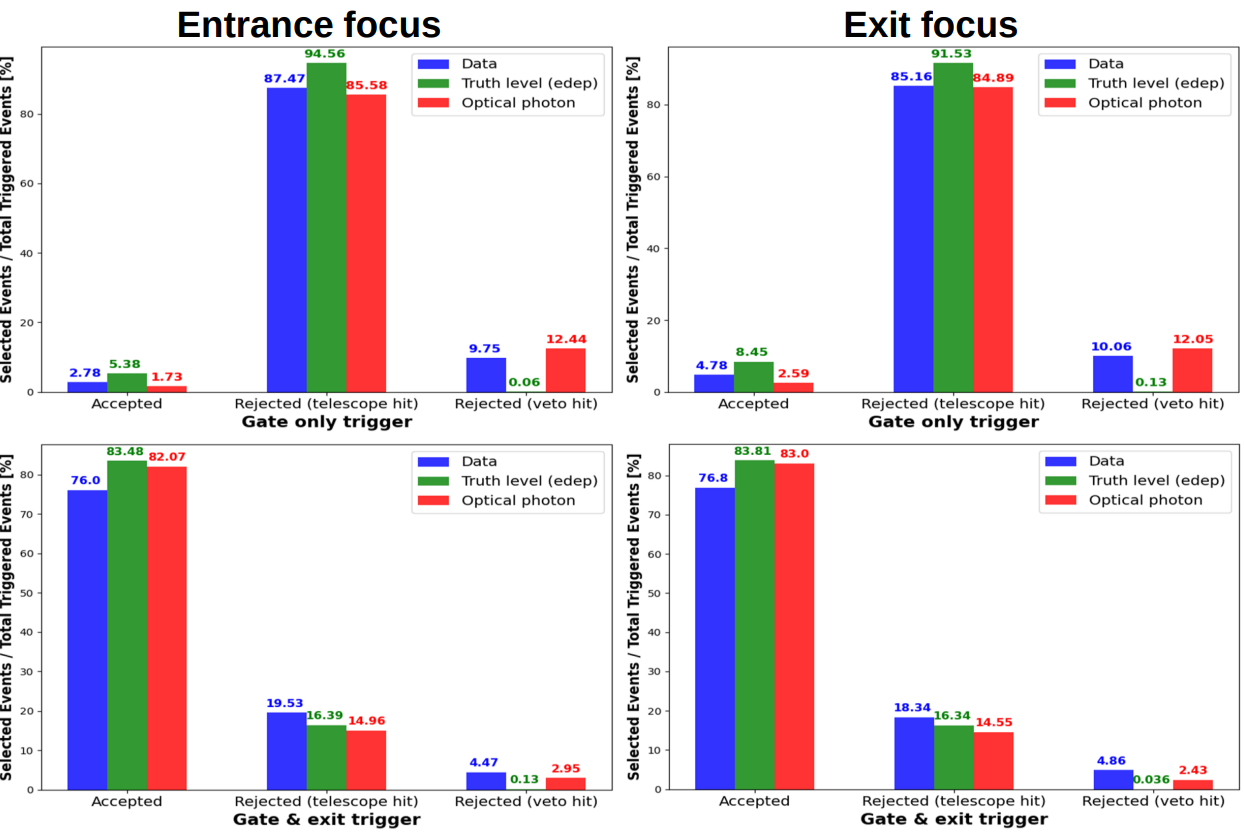
\includegraphics[width = 0.95\textwidth]{Figures/muEDM_Nov2022/shanghai_summary.png}
                \caption[]{Summary of the different events for the two beam focuses and the prediction from the \gfb prediction. See the main text for the details.}
                \label{fig:muEDM:bt2022:summary}
            \end{figure}

            \noindent
            Let's now consider a particle interacting in one of the four scintillators of the telescope. 
            If the photons produced by scintillation can bleed into the neighbor scintillators, secondary hits could be measured in these.
            So a small fraction of light will be seen by the next scintillators and very little by the one opposite (looking at Fig.~\ref{fig:muEDM:bt2022:blobs:idea}, an example could be hitting A, small fraction in D and B, and even smaller in C).
            If we now look at the charge correlation between the different scintillators, we find some interesting pattern.\\ 
            Looking at the correlation in a neighbor channel (A and B), we find a 4-dot pattern, the central graph of Fig.~\ref{fig:muEDM:bt2022:blobs:idea}. A hit in:
            \begin{outline}
                \1[A] will deposit charge in A and some in B - yellow
                \1[B] will deposit charge in B and some in A - green
                \1[C] will deposit some in B and little in A - blue
                \1[D] will deposit some in A and little in B - gray
            \end{outline} 
            If we now look at the correlation with the opposite scintillator (C), we find a different pattern, the right graph of Fig.~\ref{fig:muEDM:bt2022:blobs:idea}.
            A hit in:
            \begin{outline}
                \1[A] will deposit charge in A and little in C - yellow
                \1[C] will deposit charge in C and little in A - blue
                \1[B/D] will deposit some in A and some in C - greeen
            \end{outline} 
            These structures are the result of the optical crosstalk between scintillators so we expect these to be present in the Shanghai version of the telescope, but not in the Pisa one, having small gaps due to the gluing.
            The expectations are in line with the data, as shown in Fig.~\ref{fig:muEDM:bt2022:blobs:pisa} and Fig.~\ref{fig:muEDM:bt2022:blobs:shanghai}. 
        \begin{figure}   
            \centering
            \subfloat[Sketch to explain the correlation patterns between the charges of the different scintillators in the telescope in case of crosstalk. The scintillators are color-coded to aid understanding the patterns.]{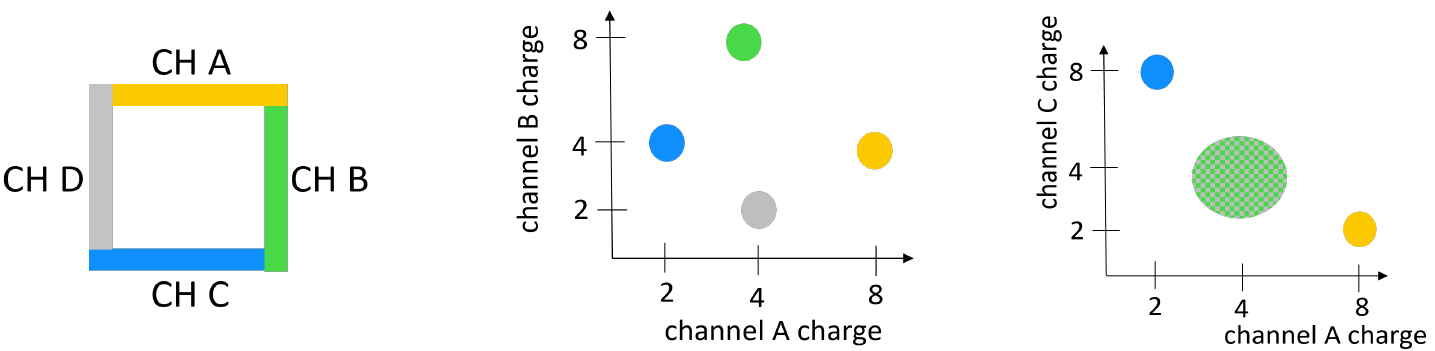
\includegraphics[width=0.9\textwidth, keepaspectratio]{Figures/muEDM_Nov2022/telescope_blobs.png}\label{fig:muEDM:bt2022:blobs:idea}}\\
            \subfloat[In the case of the telescope from Pisa, the double readout and modular style created small gaps between the scintillators. The result is that no optical crosstalk is expected nor found.]{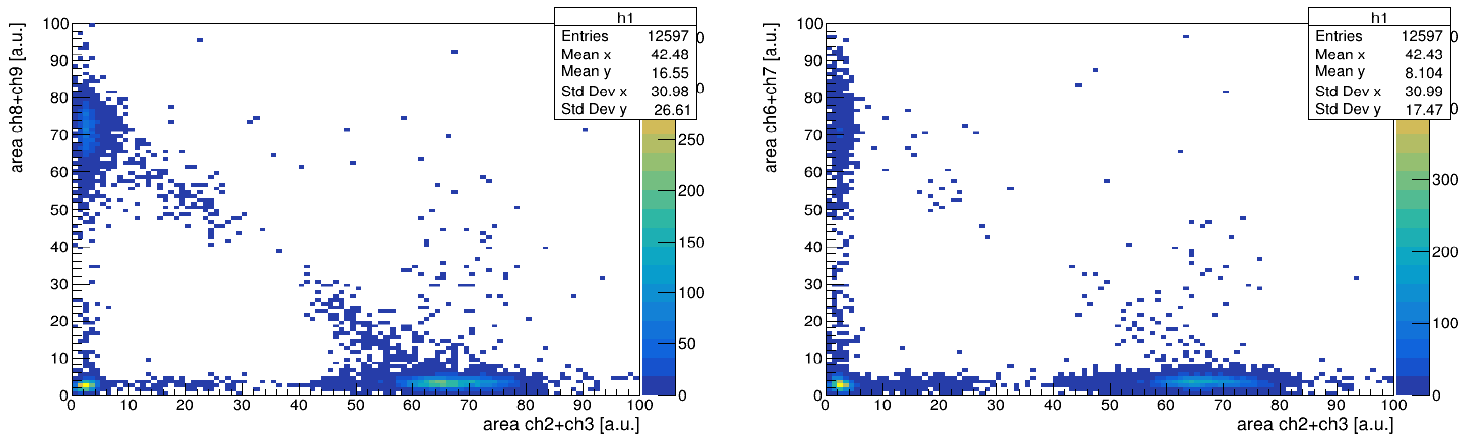
\includegraphics[width=0.9\textwidth, keepaspectratio]{Figures/muEDM_Nov2022/pisa_blobs.png}\label{fig:muEDM:bt2022:blobs:pisa}}\\
            \subfloat[In the Shanghai telescope, the scintillators are in contact. The result is the appearance of the correlation structures. These are in agreement with the expectations and nicely reproduced by the simulations.]{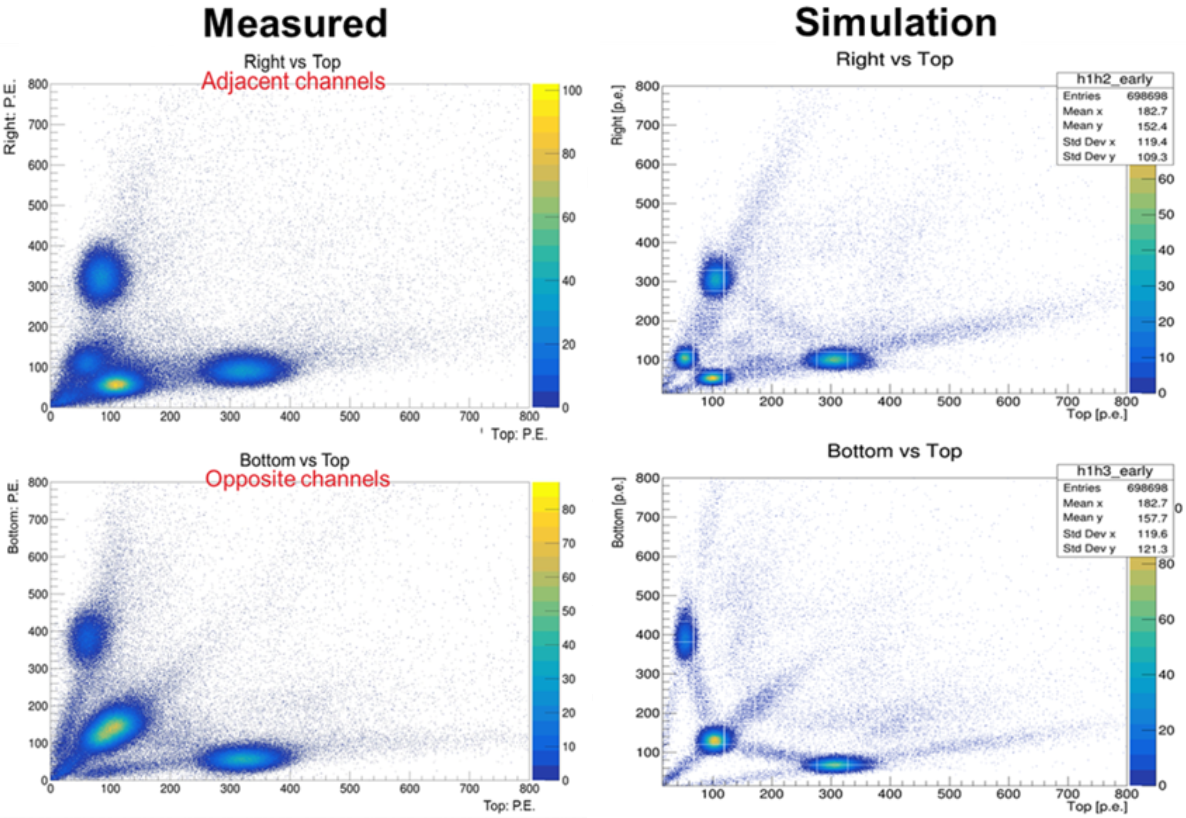
\includegraphics[width=0.9\textwidth, keepaspectratio]{Figures/muEDM_Nov2022/shanghai_blobs_g4.png}\label{fig:muEDM:bt2022:blobs:shanghai}}            
            \caption[muEDM:2022 optical crosstalk]{In case optical crosstalk is present, the correlation of the charges measured by the different scintillators show interesting patterns. These are expected and found in the Shanghai telescope, and not in the Pisa version, due to small gaps in the system.}
            \label{fig:muEDM:bt2022:blobs}
        \end{figure}

\status{review}
\section{Beamtime 2023: TOF and Multi readout entrance}
\label{sec:muEDM:beamtime2023}
    In this section, we present the experimental setup along with the first preliminary results of the test beam measurement in $\pi E1$ in December 2023. 
    The main goal of this test beam was to study the systematic effect of a change in the momentum of injected muons for magnetic fields with different polarities and magnitudes. 
    For this purpose, we focused on the measurement of the time of flight~(ToF) of muons as they pass through the vacuum of an injection channel that acts as a magnetic shield permitting a low magnetic-field path into the bore of the solenoid. 
    At the same time, different detectors were tested, such as the beam monitor and ToF detector prototypes of varying scintillator thicknesses, between \SIrange{25}{200}{\micro\meter}.

    \status{review}
    \subsection{Data taking}
        Let's start by describing the setup used during this beam time.
        The idea was to have two injection channels: inject the beam on the top line, then invert the magnetic field and shift the whole apparatus vertically to inject from the bottom line.
        Due to the delay of the height-adjustable magnet support, we could only use one channel.
        Additionally, given the studies on SC injections (Sec.~\ref{sec:muEDM:injection}) were still ongoing, we opted for magnetic steel, which would shield up to \SI{0.8}{T}. 
        For this reason, we limited the magnet field to $-750<B<750$ mT, so that the fringing fields could not behave as magnetic mirrors, rejecting the incoming muon, or deflecting them too much from the trajectory.
        Figure~\ref{fig:TB2023murTubes} shows a simulation of the relative permittivity of the injection tube for three different nominal magnetic-field values in the center of the solenoid bore. With a field of \SI{750}{\milli\tesla} the relative permittivity of the tubes remains above 10 indicating no or only low saturation along the tube. Moreover, as seen in Figure~\ref{fig:TB2023FieldInTube}, with a field of \SI{750}{\milli\tesla} the magnetic field strength in the middle of the tube is below \SI{100}{\milli\tesla} for $\sim$\SI{98}{\%} of the length of the injection tube. 
        By setting the PSC magnet to produce a magnetic field of \SI{750}{\milli\tesla} inside its bore, a shielding factor of almost two along the center axis of the injection tube is expected.
        The expected stress for these injection channels is significant and for this reason, a proper holding structure was developed and we opted for \textit{dummy}-injection tubes to mitigate the stress generated on the magnet.
        The \ansys structural simulation, the CAD design of the holder, and the overall setup are shown in Fig.~\ref{fig:muEDM:2023:setup}.
        The injection channel was vacuumed and sealed with \SI{35}{\micro\meter} \mylar foils.
        At both ends of the injection channels detector modules were connected: three upstream (Veto, BeamMonitor, TOF in) and one downstream (TOF out), all described in the following paragraphs.
        The DAQ system was the WaveDAQ standalone board, able to digitize the waveforms of each channel up to 5 GSample/s. 
        The WaveDAQ provides also the power for the MPPC, up to $\approx\SI{220}{V}$ per channel. 
        The trigger configurations were also set using the GUI interface of WaveDAQ. 

        \begin{figure}
            \centering
            \subfloat[Relative permittivity in the magnetic steel]{
            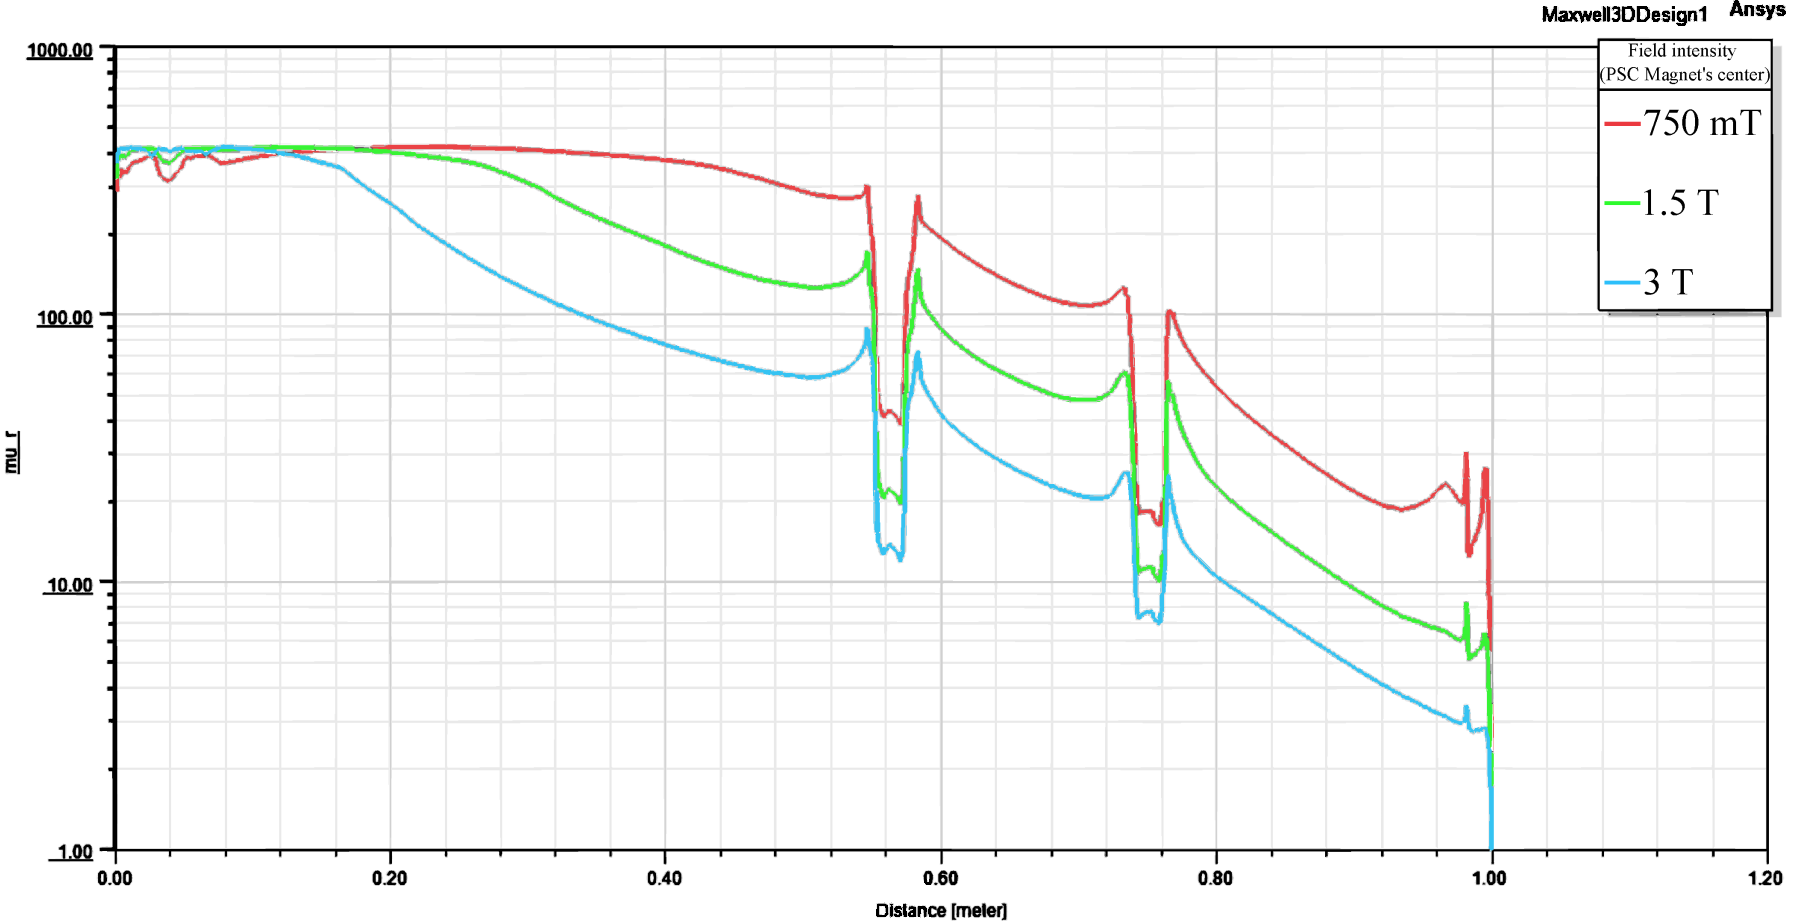
\includegraphics[width=0.9\textwidth]{Figures/muEDM_Dec2023/SaturationLowField.png}
            \label{fig:TB2023murTubes}}
            \\
            \subfloat[Magnetic field strength along the middle of the tube]{
            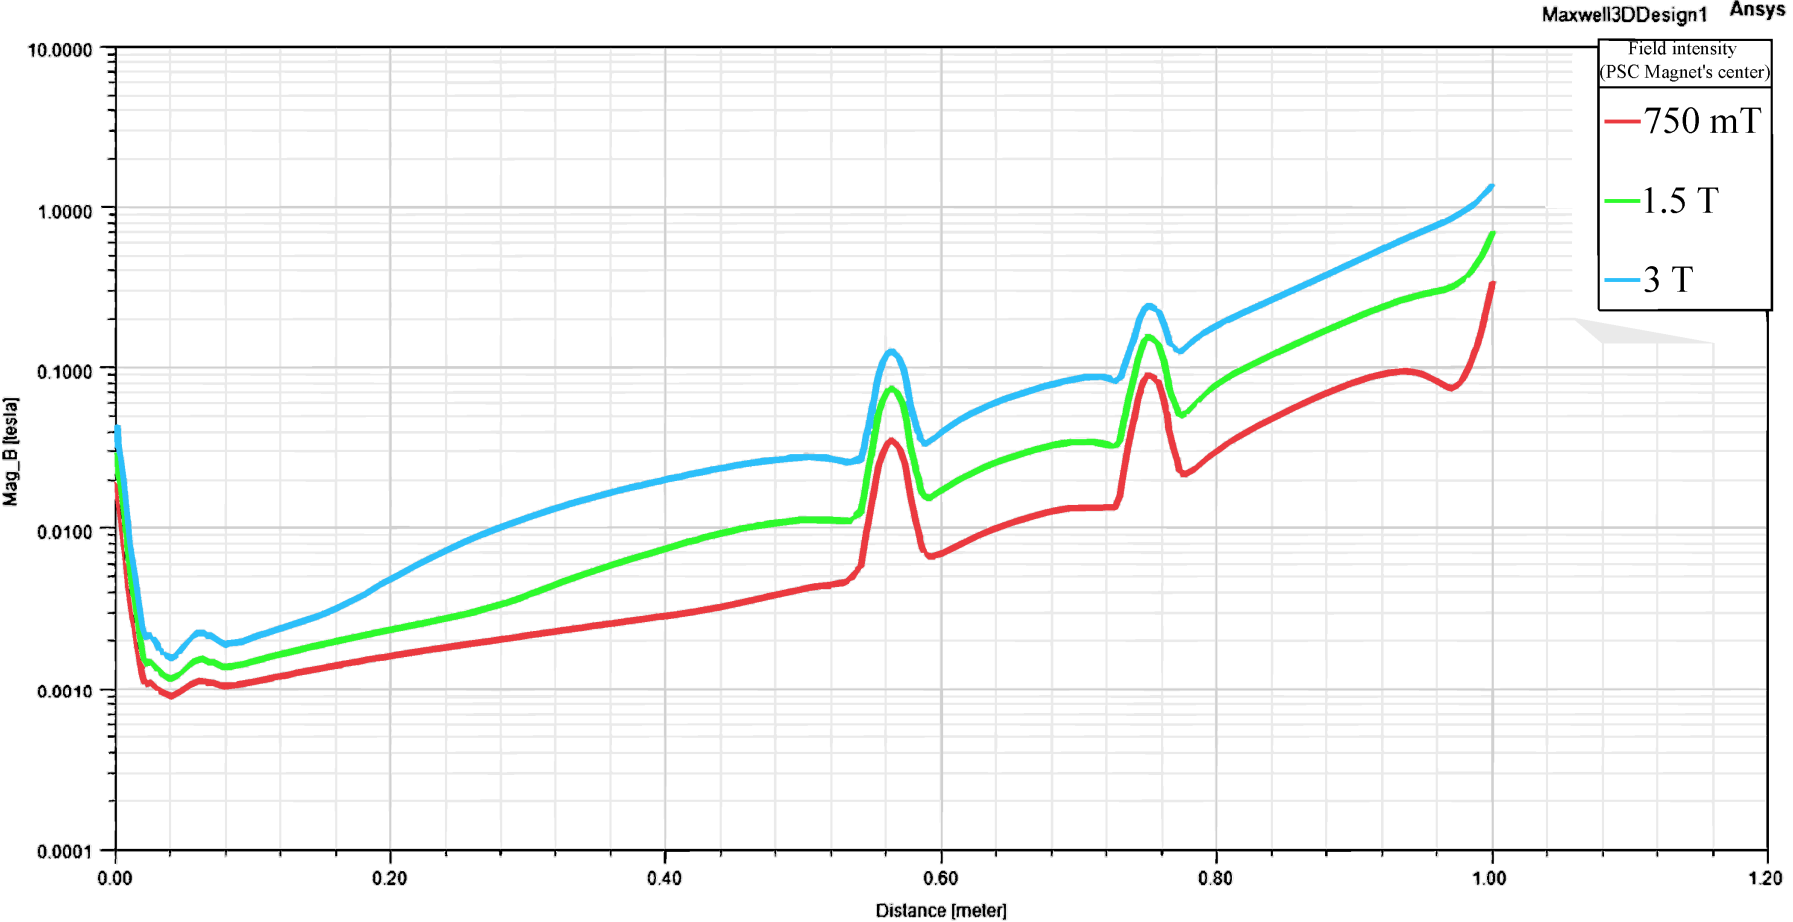
\includegraphics[width=0.9\textwidth]{Figures/muEDM_Dec2023/FieldTubesSim.png}
            \label{fig:TB2023FieldInTube}}
            \caption{Simulation results for different nominal magnetic fields at the center of the PSC solenoid. (a)~shows the relative permittivity of the injection tubes as a function of the distance along the tube, starting from the upstream position and going towards the downstream position inside the bore of the PSC magnet. (b)~shows the magnetic field strength along the middle of the injection tube. Note that the two significant features are a result of a reduced wall thickness of the steel tube at these positions, for the mechanical support.}
            \label{fig:TB2023FieldStrengthTubes}
        \end{figure}	
        \begin{figure}
            \centering
            \subfloat[The stress of the setup and ghost image of the deformation caused ($\times100$).]{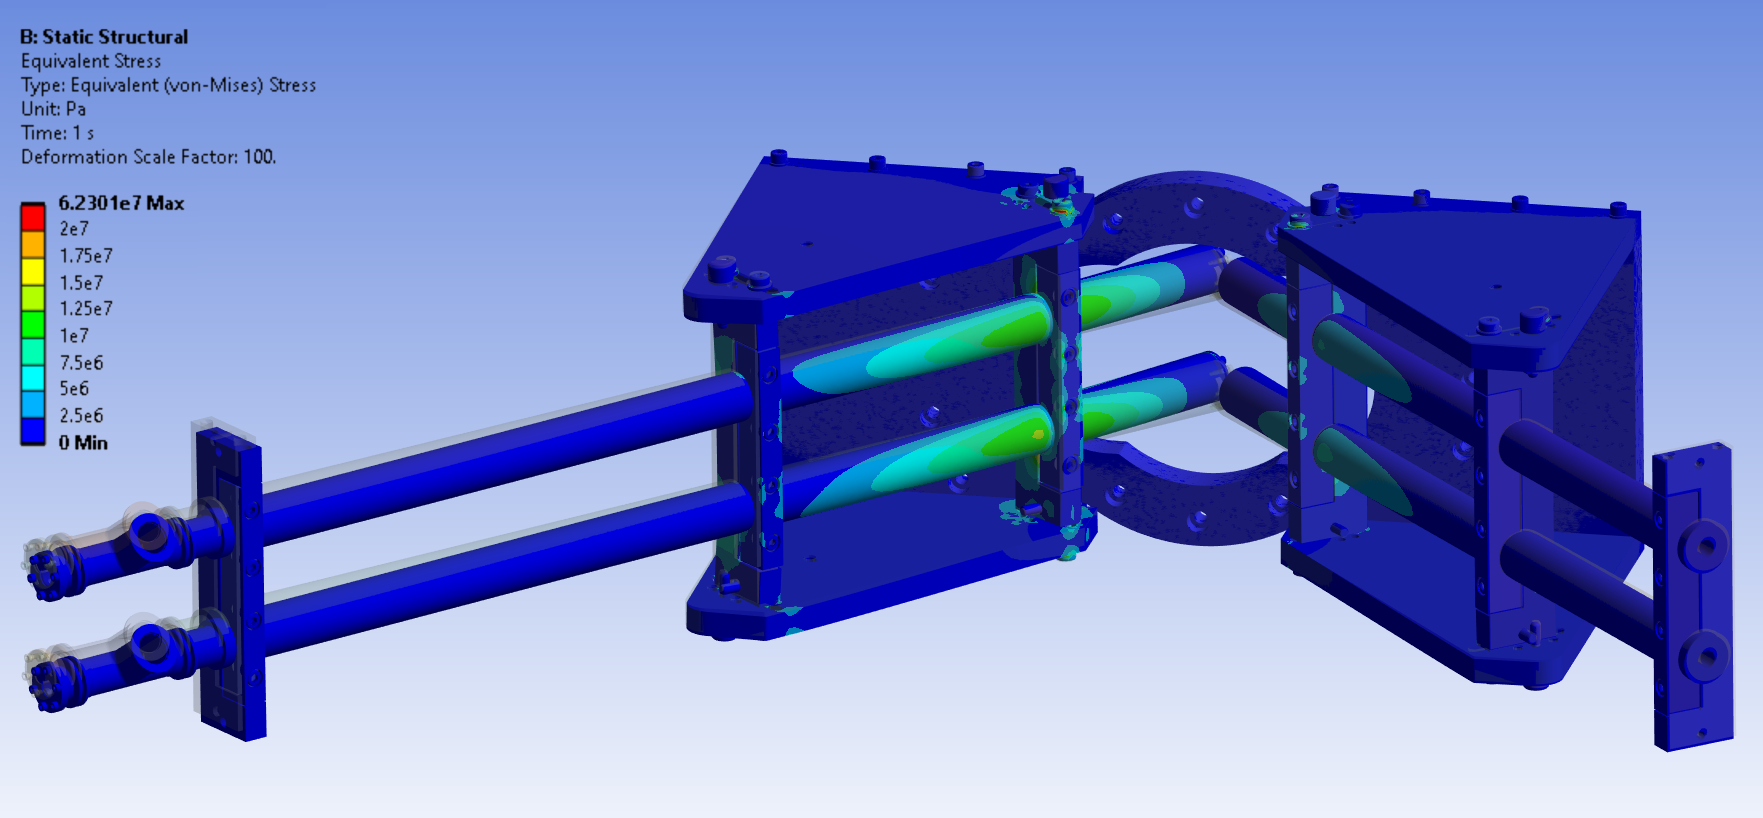
\includegraphics[width=0.8\textwidth]{Figures/muEDM_Dec2023/ForceSim.png}}\\
            \subfloat[CAD design of the whole setup.]{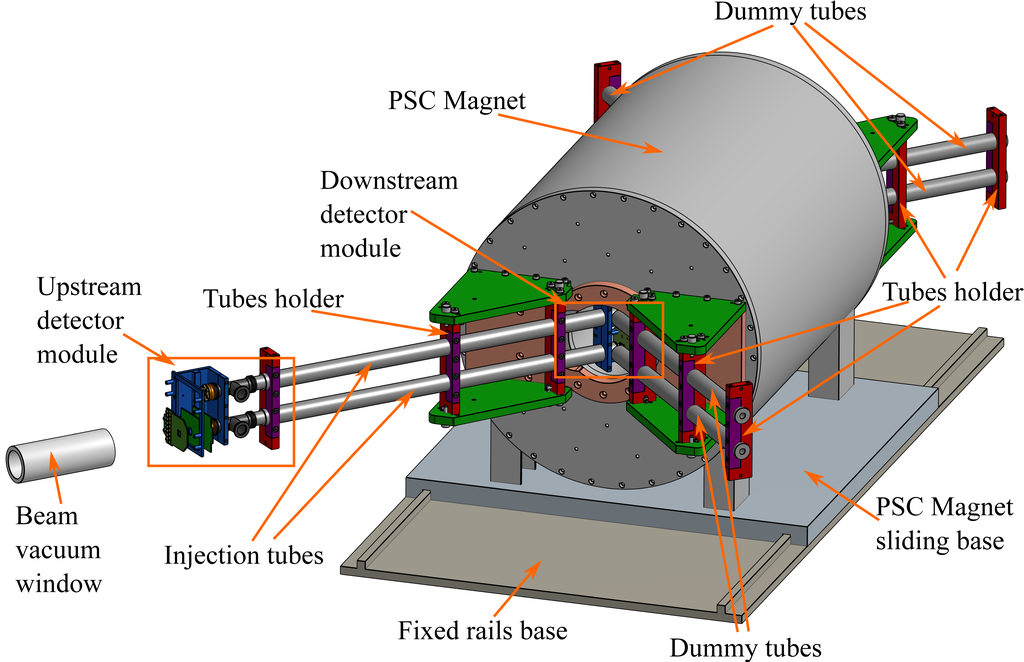
\includegraphics[width=0.8\textwidth]{Figures/muEDM_Dec2023/AssemblyTestBeam2023.png}}\\
            \subfloat[CAD detail of the US detectors.]{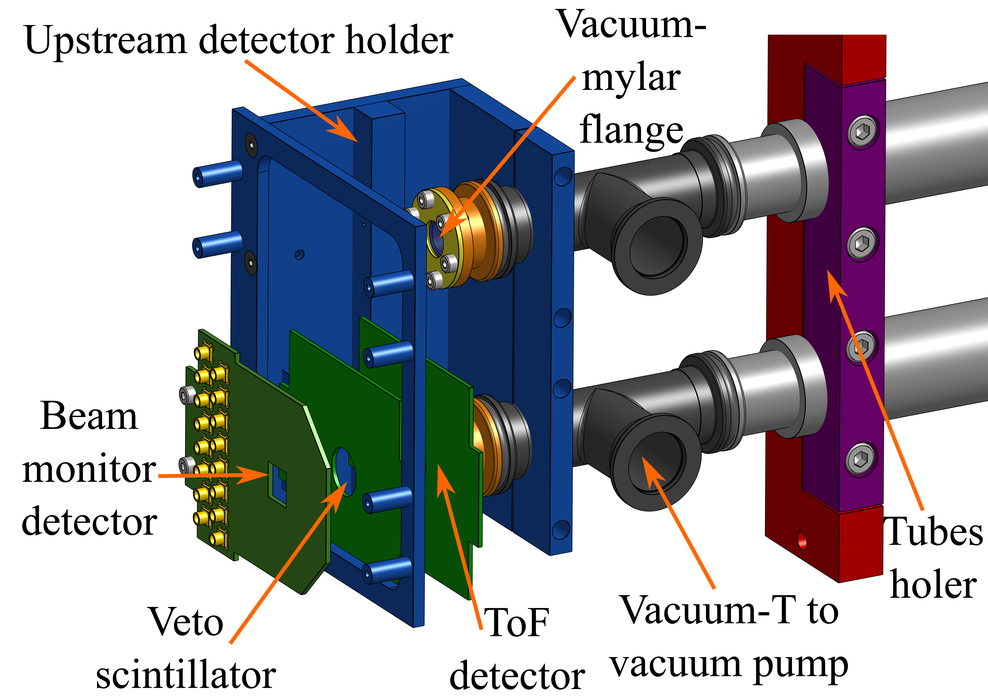
\includegraphics[width=0.45\textwidth]{Figures/muEDM_Dec2023/AssemblyTestBeam2023US.png}}\hfill
            \subfloat[CAD detail of the DS detectors.]{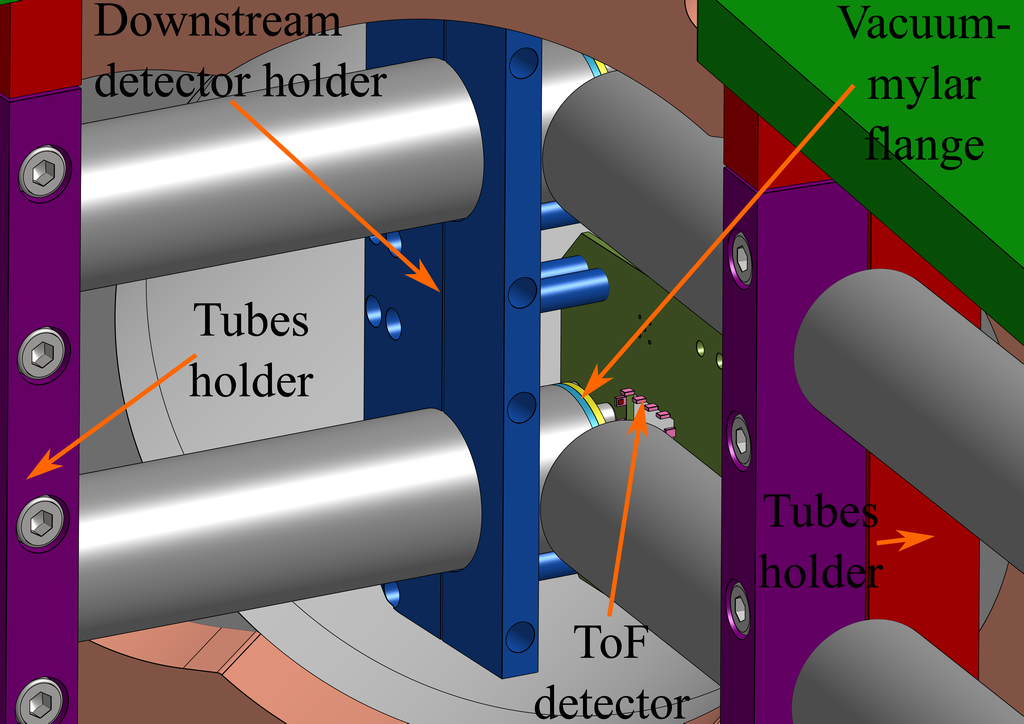
\includegraphics[width=0.45\textwidth]{Figures/muEDM_Dec2023/AssemblyTestBeam2023DS.png}}
            \caption{The support structure was developed to reduce stresses to the injection channel and the PSC magnet: \textbf{(a)} shows the \ansys studies, \textbf{(b)} the whole setup, \textbf{(c)} and \textbf{(d)} the detail of the US and DS detectors.}
            \label{fig:muEDM:2023:setup}
        \end{figure}


        \paragraph{Beam and Beam Monitor}
        The first thing was to measure the lateral phase space to later match the simulations.
        This can be calculated from measurements of the beam profile taken over a scan of the current in the last two quadrupoles. 
        The profiles were measured using a $2\times\SI{2}{mm\squared}$ pill counter moved by an $xy$-scanner for each implemented beam configuration.
        After removing the pill, the first item in the setup was the Beam Monitor, a squared detector made of scintillators arranged to have a squared hole.
        The aim of this detector, as outlined in Ch.~\ref{ch:muEDM}, where the details of the working principles were previously discussed, is to center the beam.
        Two monitors with different segmentation and scintillator tile shapes were tested.
        One consisted of eight rectangular tiles, while the other consisted of four triangular tiles per layer. 
        Additionally, two orientations at a rotation of $0^{\circ}$ and $180^{\circ}$ around the beam axis were compared to check the performance of individual tiles. 
        Finally, the measurements were performed at different magnetic fields generated by the PSC magnet to map the deflection of the beam spot at the entrance of the injection channel.
        
        \paragraph{Time Of Flight (TOF)}
        Following the beam monitor, two scintillators are used to evaluate the time of flight.
        The idea is to use thin scintillators to reduce the multiple scattering.
        From the previous beamtime, we know we can use $\SI{100}{\micro m}\divisionsymbol\SI{200}{\micro m}$ achieving an intrinsic time resolution of $\upsigma_{int}\approx\SI{300}{\micro s}$.
        The aim here is to evaluate the momentum spread of the beam by measuring the TOF.
        The difference in momentum translates into the difference in time of the scintillator signals $\Delta t$. 
        The distribution of $\Delta t$ is the convolution of the momentum distribution and the intrinsic time resolution of the system.
        Assuming a Gaussian distribution for the beam momentum, centered around \SI{28}{MeV/c} and having spread 1\%, 3\%, and 5\%, we can evaluate the $\Delta t_{measured}$ for different distances.
        In Fig~\ref{fig:muEDM:bt2023:TOFPython} the expected distributions for $1\%$ spread and $\upsigma_{int}\approx\SI{300}{\micro s}$, while the \textit{std. dev.} of the obtained distributions is shown as a function of distance for 3\% and 5\%.
        From these estimations we can conclude a 1\% momentum spread, with the given $\upsigma_{int}$ and reasonable distances, cannot be appreciated. 
        The situation seems different for 3\% and 5\%.
        Figure~\ref{fig:TB2023ToFPhoto} shows one of the ToF prototypes fabricated in 2023, while it was being mounted to the injection tubes. \\

        \noindent
        The coincidence of different channels per detector was studied, to decrease the threshold, increase the sensitivity of each detector, and reach the maximum efficiency by comparing combinations of different prototypes under test beam conditions. 
        As the beam characteristics and the momentum of the muons were essentially constant, it was possible to test the effects of the magnetic field ``handedness'', CW vs.\ CCW storage of the muons inside the storage magnet, on the momentum and muon trajectory along the injection channel by measuring the ToF between upstream~(US) and downstream~(DS) detector. 
        Measurements with different magnetic field strengths and polarities were performed.
        The changes in the magnetic field were performed by sweeping between the maximum magnetic-field magnitudes of $\pm$\SI{750}{\milli\tesla}, in such a way as to also be sensitive to possible hysteresis effects.
        \begin{figure}
            \centering
            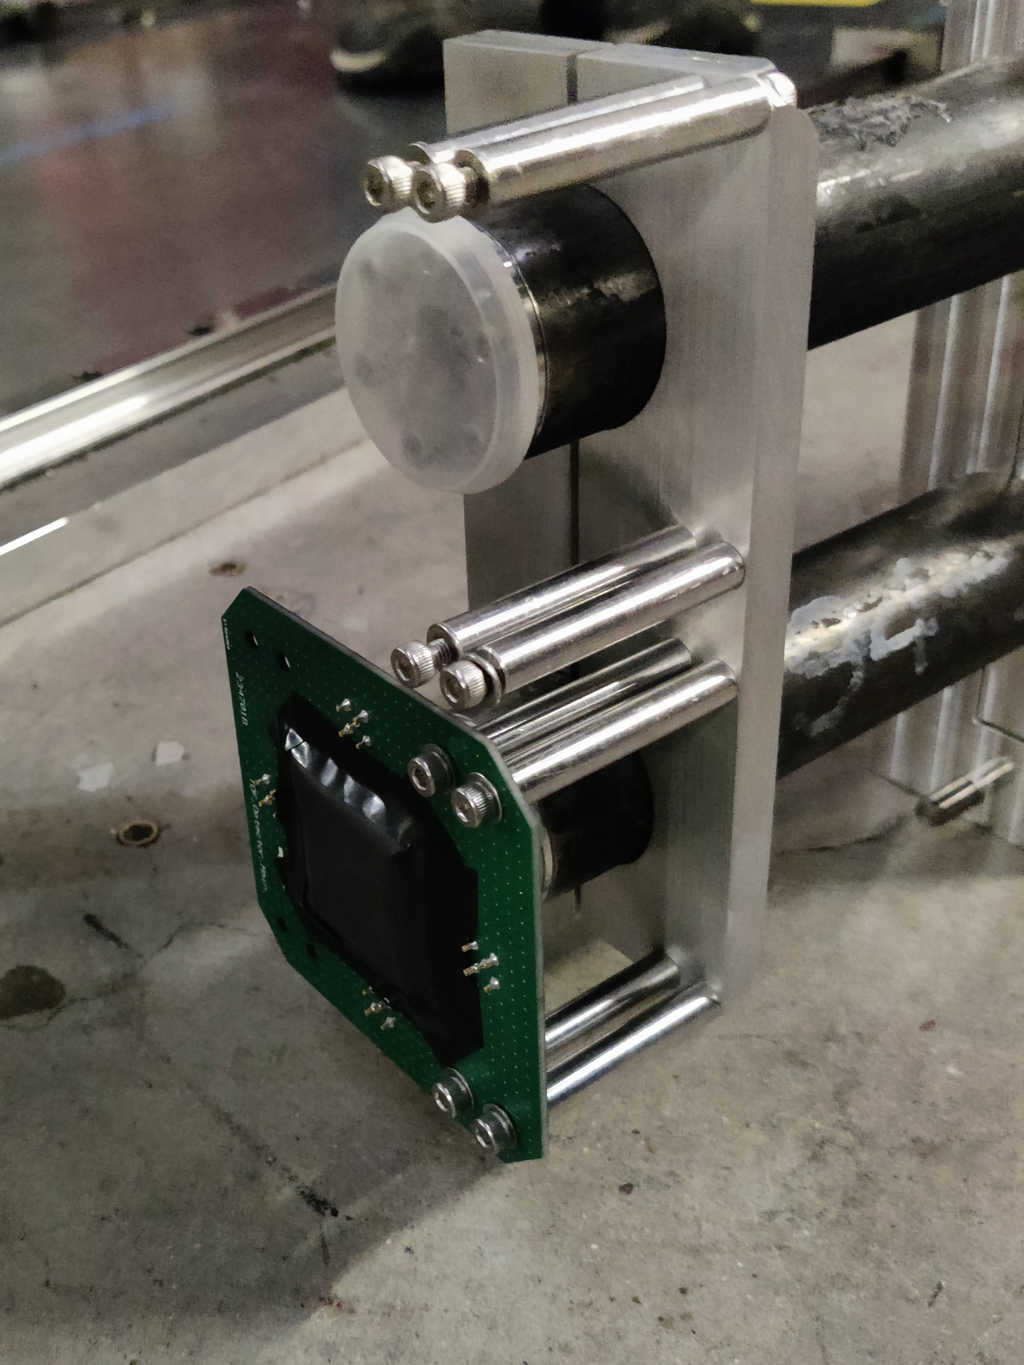
\includegraphics[width=0.5\textwidth]{Figures/muEDM_Dec2023/IMG_20231209_225342Small.png}
            \caption{One of the ToF detector prototypes fabricated in 2023 with four readout channels. The detector is mounted on the downstream detector module which is attached to the injection tubes.}
            \label{fig:TB2023ToFPhoto}
        \end{figure}
        
        \begin{figure}
            \centering
            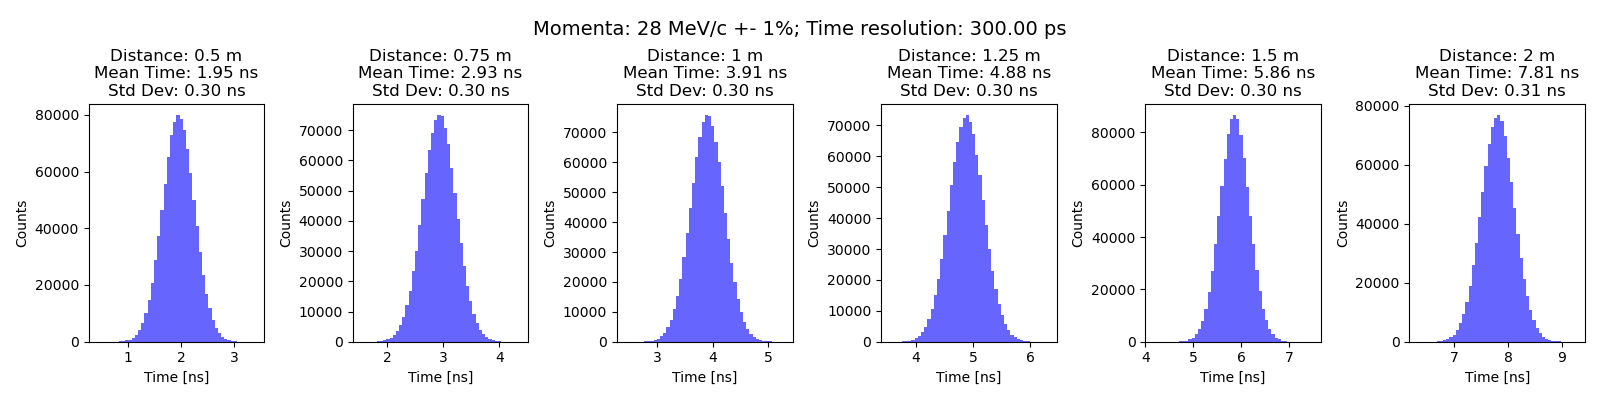
\includegraphics[width=\textwidth]{Figures/muEDM_Dec2023/histo_28_1_300.png}\\
            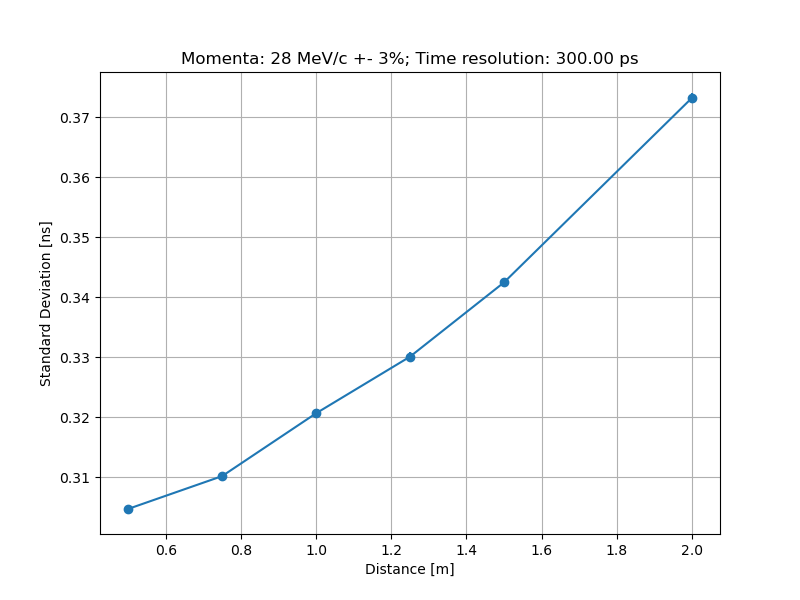
\includegraphics[width=0.49\textwidth]{Figures/muEDM_Dec2023/trend_28_3_300.00.png}
            \hfill
            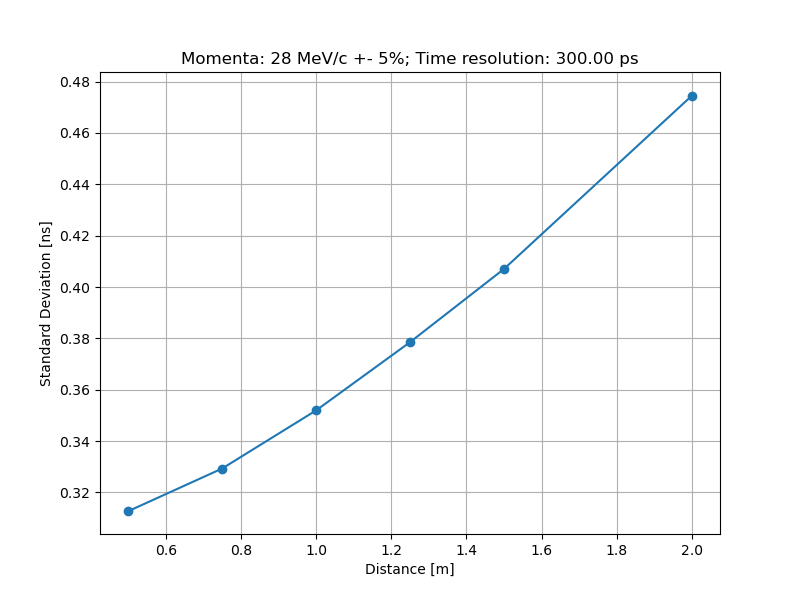
\includegraphics[width=0.49\textwidth]{Figures/muEDM_Dec2023/trend_28_5_300.00.png}
            \caption[muEDM 2023: TOF momentum spread.]{A simple Python simulation to evaluate the resolution for the TOF for different distances, momentum spread, and time intrinsic resolution of the couple of scintillators used. For $\upsigma_{int}=\SI{300}{ps}$ we do not appreciate a 1\% spread in momentum while we have the sensitivity for 3\% and 5\%.}
            \label{fig:muEDM:bt2023:TOFPython}
        \end{figure}

        \paragraph{Multi-readout \textit{gate}}
        A cardinal point was the implementation of four independent readout channels for the new thin scintillators. 
        This was discussed earlier (Sec~\ref{sec:muEDM:beamtime2022}) and is linked to the necessity of lowering the threshold while keeping a low dark rate.
        A picture during the soldering and the CAD design are shown in Fig.~\ref{fig:muEDM:bt2023:TOF:picture}.
        We took data with mixed (old 1ch and new 4ch) and matched (new 4ch and new 4ch) setups.
        This allowed us to benchmark the new detectors.
        
        \begin{figure}
            \centering
            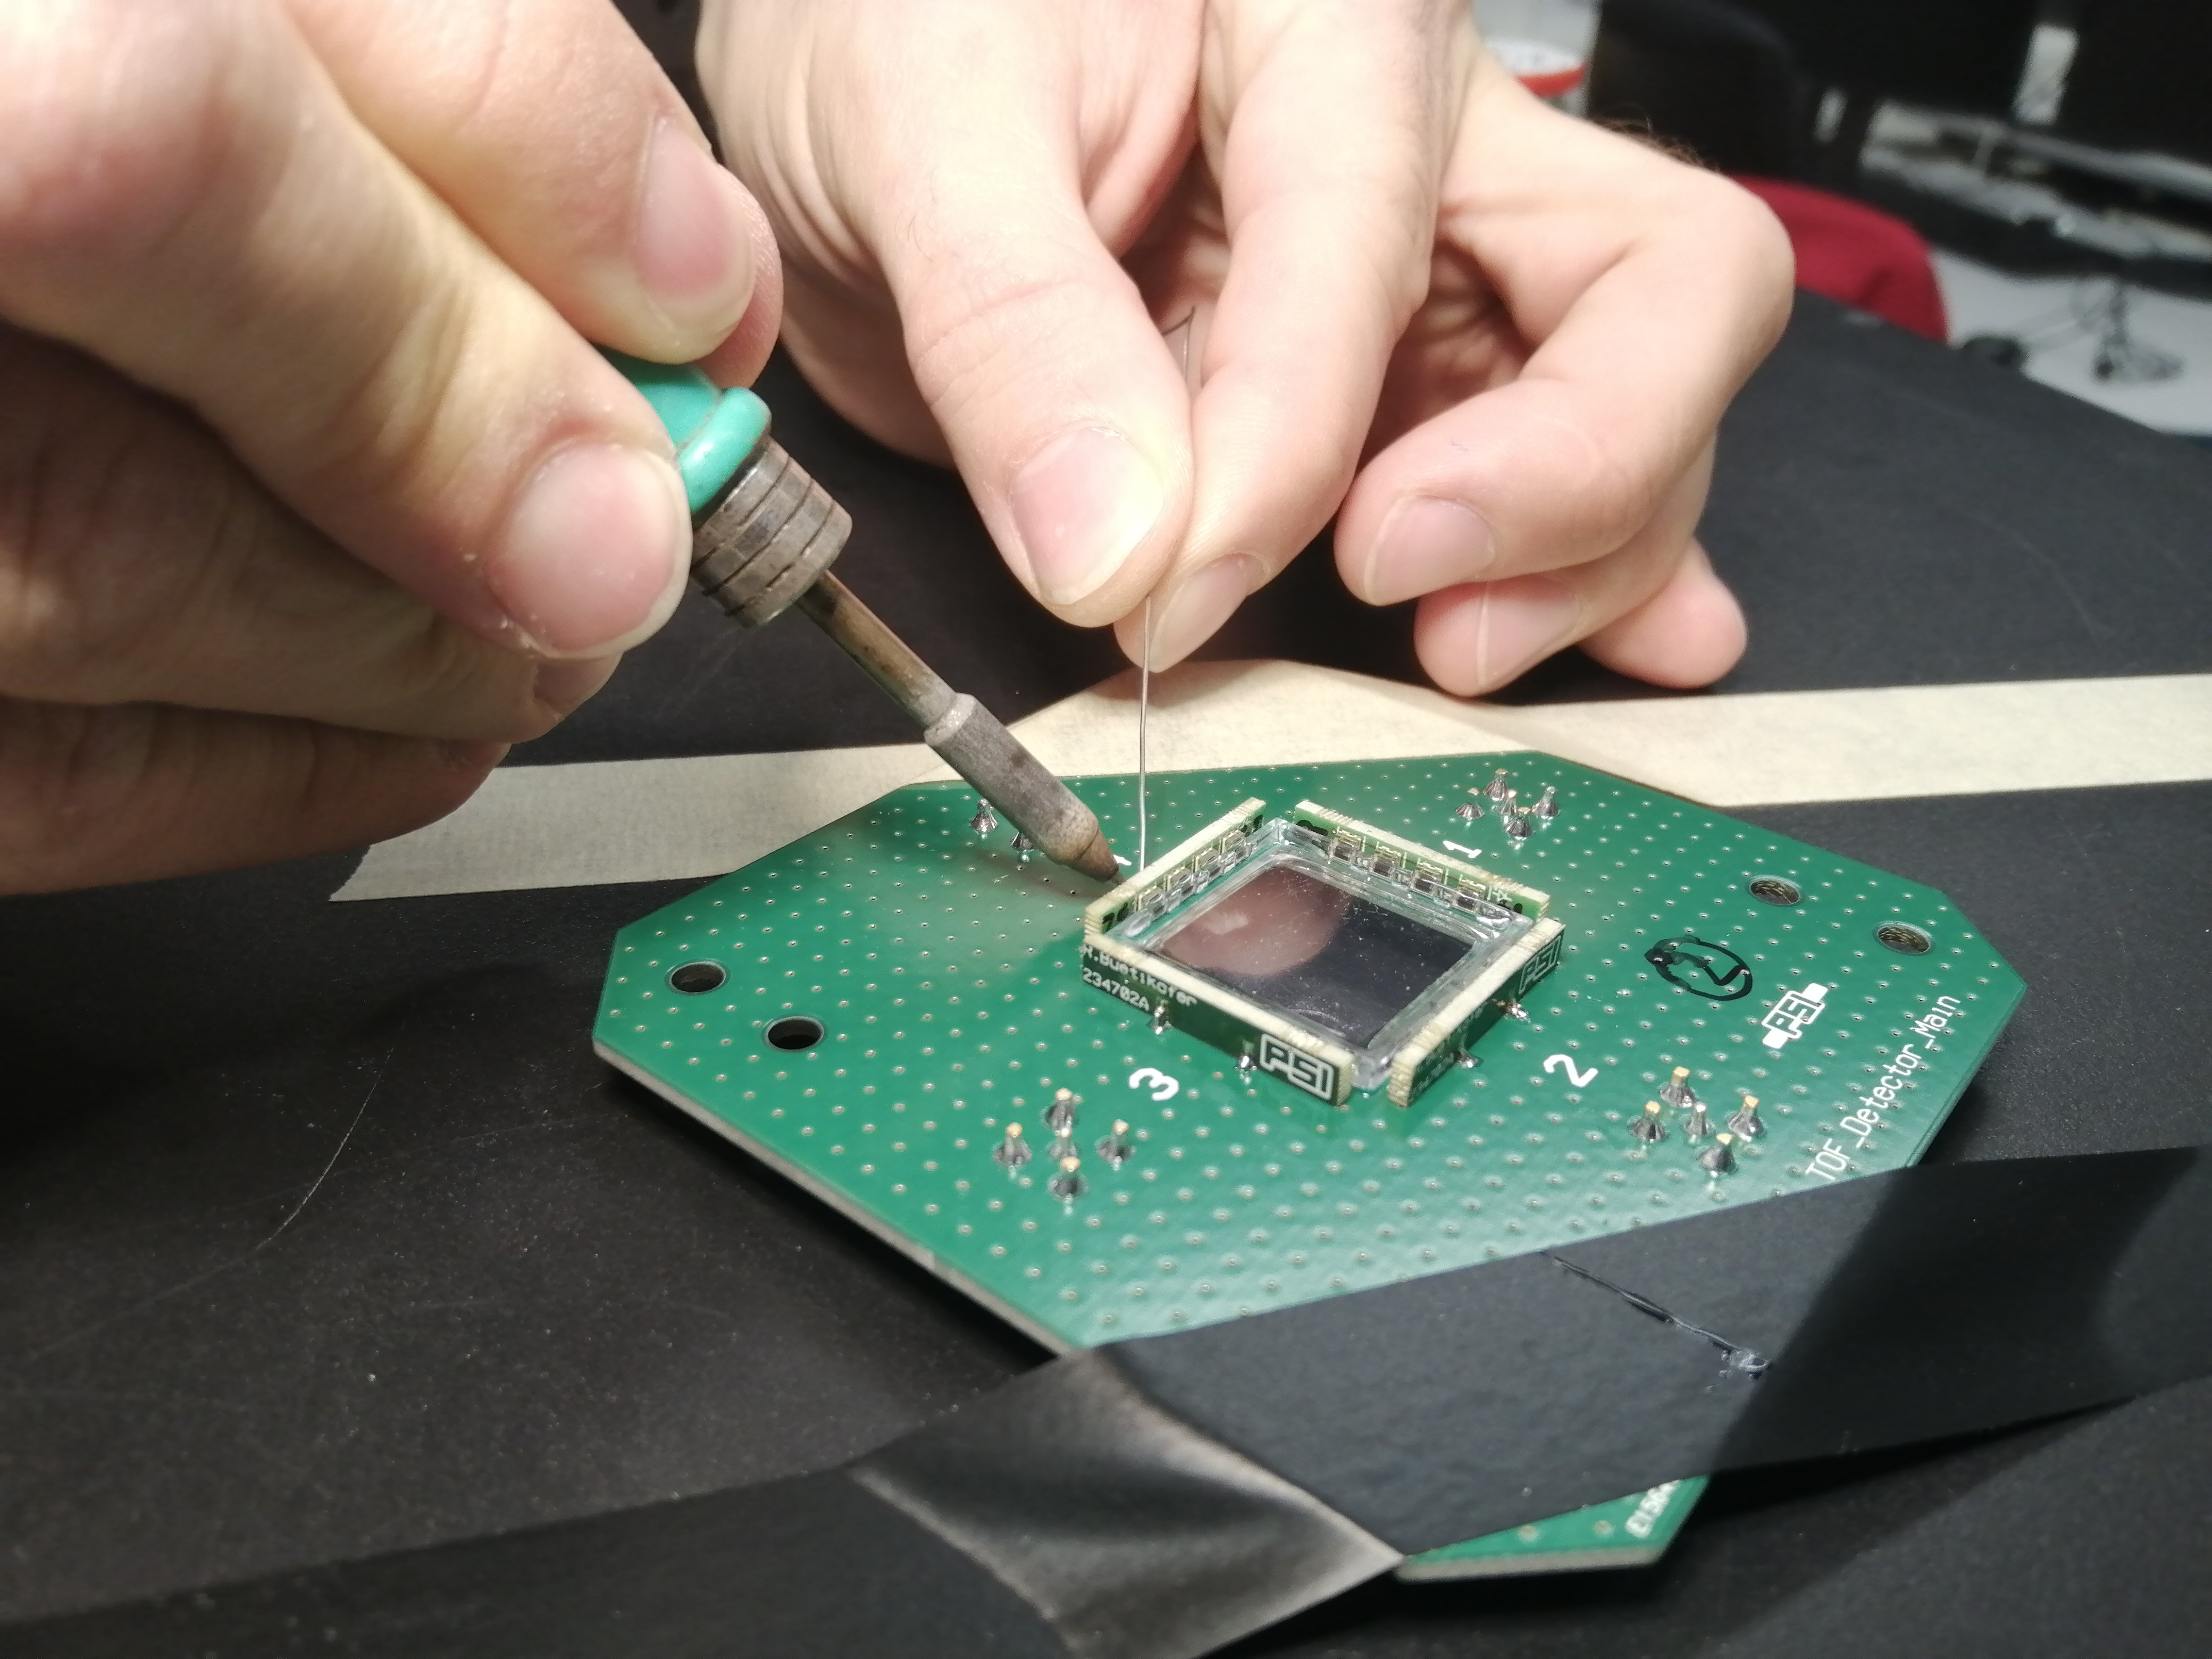
\includegraphics[height=5cm]{Figures/muEDM_Dec2023/TOF_soldering.jpg}
            \includegraphics[height=5cm]{Figures/muEDM_Dec2023/TOF_CAD.png}
            \caption[muEDM 2023: TOF detector soldering.]{A picture of the TOF detectors used during the 2023 December beam-time. Thin scintillators (50 and \SI{100}{\micro m}) read on four sides by four SiPMs.}
            \label{fig:muEDM:bt2023:TOF:picture}
        \end{figure}

        \paragraph{Efficiency and calibration}
        Along the $\pi E1$ beamline, a separator akin to a Wien filter is employed to discriminate between muons and pions by adjusting the relative strengths of magnetic and electric fields. 
        When both fields are set to zero, particles with the desired momentum (in our case, \SI{28}{MeVc/}) pass through the separator and reach the experiment. 
        We utilized this functionality to calibrate the Time of Flight (ToF) setup by measuring the ToF of positrons traveling near the speed of light.
        Another setup was dedicated to evaluating the relative efficiency and intrinsic time resolution of the detectors. Two detectors were positioned back-to-back with minimal spacing (a few millimeters), and this configuration was repeated for all possible detector pairs.

    \status{review}
    \subsection{Data analysis}
        \paragraph{Beam Monitor}
        The two tested versions were the 4 and 8-segmented variants.
        Using the WaveDREAM board, the 16 different channels had a threshold adjusted so to keep the dark noise manageable.
        Ideally, with the beam on, the front \SI{2}{mm} scintillators would distinguish the particle ID creating two peaks but this was not the case for all channels (Fig.~\ref{fig:BeamMonRect_pulsesDefaultThresh}). 
        Optical coupling and soldering of these channels are under test.
        At this point, the threshold of the front layer was changed to select muons.
        Two triggers were used during data-taking: requiring a hit in the channel of interest, regardless of all other 15 channels, and requiring a hit in the tile of interest, while vetoing a hit in all the 5 mm channels.
        The beam monitor position and B field scan were repeated by flipping the detector by \SI{180}{\deg}.
        Examples of the measurements taken for the two versions are in Fig.~\ref{fig:BeamMonRect_positionScan} and Fig.~\ref{fig:BeamMonTriang_positionScan}. 
        Overall the 8-segmented version behaved as expected while the other presented a `hot'-channel.
        The analysis is still ongoing but the positioning of the beam seems to be sub-optimal. 
        For example, the 4-segmented version misplaced the beam center by \SI{6.3}{mm}.


        \begin{figure}
            \centering
            \includegraphics[width=0.49\textwidth]{Figures/muEDM_Dec2023/Corner_overlay_TueHVset_rect.png}
            \includegraphics[width=0.49\textwidth]{Figures/muEDM_Dec2023/Middle_overlay_TueHVset_rect.png}
            \caption{Charge integral of the 8-segmented beam monitor as extracted online in WaveDAQ GUI. Left: overlay of all the corner 2~mm thick tiles. Right: overlay of all the middle 2~mm thick tiles. The peak on the right corresponds to positrons, while the broader peak on the left corresponds to muon energy depositions.}
            \label{fig:BeamMonRect_pulsesDefaultThresh}
        \end{figure}
        
        \begin{sidewaysfigure}
            \centering
            \includegraphics[width=0.95\textwidth]{Figures/muEDM_Dec2023/BeamMonRect_scanData2023.png}%
            \caption{The online rates in kHZ in 2~mm thick tiles of the 8-segmented beam monitor. The rates were recorded for three x-positions left and right of the nominal detector position (the center images). The top two rows show the rates for the beam monitor in "0 deg" position, while the bottom two rows show the data for the "180 deg" rotated monitor. Two rows for each detector rotation correspond to the two trigger configurations (see text), with the upper row being just the rate of a channel, and the bottom row requiring a hit in the channel and no hits in the thicker back scintillator plane. The beam is entering the image plane along the line of sight.}
            \label{fig:BeamMonRect_positionScan}
        \end{sidewaysfigure}
        
        \begin{sidewaysfigure}
            \centering
            \includegraphics[width=0.9\linewidth]{Figures/muEDM_Dec2023/BeamMonTriang_scanData2023.png}%
            \caption{The online rates in kHZ in 2~mm thick tiles of the 4-segmented beam monitor. The rates were recorded for two x-positions left and right of the nominal detector position (the center images). The top two rows show the rates for the beam monitor in "0 deg" position, while the bottom two rows show the data for the "180 deg" rotated monitor. Two rows for each detector rotation correspond to the two trigger configurations (see text), with the upper row being just the rate of a channel, and the bottom row requiring a hit in the tile (with a signal in both channels) and no hits in the thicker back scintillator plane. The beam is entering the image plane along the line of sight.}
            \label{fig:BeamMonTriang_positionScan}
        \end{sidewaysfigure}

        \paragraph{TOF scintillators}
        Two TOF detectors per scintillating foil thickness (\SI{100}{\micro m} and \SI{50}{\micro m}) have been tested, for a total of four detectors, in different combinations. 
        The beamtime aimed to measure the detection efficiency of each detector and its intrinsic timing resolution, as well as the time-of-flight resolution for all the possible combinations of the available detectors.
        The threshold of each channel was set to have a dark count rate of a few 100 Hz (apart from a couple of noisy channels up to 1 kHz) with the Beam Blocker closed. 
        As a reference, with the settings of our beamline, we had a typical rate of $\approx50$ KHz on the US detector.

        \noindent
        Two experimental setups have been used to extract the detector characteristics as listed above:
        \begin{itemize}
            \item the \textit{short} configuration, with the two detectors separated by less than 1 cm, along the beamline direction. 
            The first detector is the detector under test (DUT), while the second is the reference (REF). 
            This configuration can be used to extract the efficiency of the DUT, by triggering on the REF, and the intrinsic timing resolution for the detector pair under study, due to the relatively short distance between the two detectors.
            \item the \textit{long} configuration, with the two detectors mounted at the entrance and exit of the injection line. This configuration is the one used to measure the TOF.
        \end{itemize} 
        Fig.~\ref{fig:TOF_short_and_long} shows the pictures of the mounted detectors in short (left) and long (right) configurations.\\

        \begin{figure}
            \centering
            \includegraphics[width=1\linewidth]{Figures/muEDM_Dec2023/TOF_setup_assembly_in_area.png}
            \caption{The \textit{short} and \textit{long} configurations, used to extract the main parameters of the TOF detectors.}
            \label{fig:TOF_short_and_long}
        \end{figure}

        \noindent
        Detectors of the same thickness showed similar efficiency. 
        The numbers reported here refer to the mean of the two. 
        They are still preliminary and conservative but provide a reasonable overview.

        \begin{outline}
            \1 \textbf{\SI{100}{\micro m}}: A full detection efficiency (> 99\%) is measured requiring \textit{at least one fired channel}. It decreases if at least \textit{two}, \textit{three}, or \textit{four} fired channels is requested (>98\%, >96\%, >95\%).
            \1 \textbf{\SI{50}{\micro m}}: With similar requirements the efficiency measured is >87\%, >64\%, >45\%, and >40\%.
        \end{outline}\\

        \noindent
        Fig.~\ref{fig:TOF_intrinsictimeresolution100pair} shows the intrinsic time resolution for the \SI{100}{\micro m} detector pair, using a constant fraction method to extract the time of each channel. 
        A timing resolution of ~450 ps is measured if the time difference of two fixed channels is plotted (red line). 
        The timing algorithm can be easily optimized by taking advantage of the segmented detector, made of four independent channels. 
        For each event, the fastest channel on each side can be used to plot the time difference. 
        This is shown as the blue line, with a timing resolution down to ~\SI{300}{ps}. 
        The same analysis can be repeated with the two detectors mounted in the long configuration, with the results shown in Fig.~\ref{fig:TOF_TOFresolutionpair} with the mean of the distribution being the TOF of the impinging particles and its resolution being the convolution of several terms, including the intrinsic timing resolution of the detector pair and the momentum spread of the particles.
        \noindent
        Although these results are very preliminary, the expected detector performances are nicely addressed and satisfy the experiment requirements.


        \begin{figure}
            \centering 
            \subfloat[Short configuration with \SI{100}{\micro m} detector pair.]{\includegraphics[width=0.5\linewidth]{Figures/muEDM_Dec2023/TOF_preliminary_shortconfiguration100pair.png}\label{fig:TOF_intrinsictimeresolution100pair}}
            \subfloat[Long configuration with \SI{100}{\micro m} detector pair.]{\includegraphics[width=0.5\linewidth]{Figures/muEDM_Dec2023/TOF_preliminary_longconfiguration100pair.png}\label{fig:TOF_TOFresolutionpair}}
            \caption{Time difference for the \SI{100}{\micro m} detector pair, mounted om the \textit{short} (a) and \textit{long} (b) configuration. In red the result of taking two fixed channels, in blue taking the first channel to be triggered in the detectors.}
        \end{figure}

        \paragraph{TOF}
        TOF measurements were taken for different detector setups and at different magnetic fields in the range of \SI{-750}{mT} to \SI{+750}{mT}. 
        The mounted detectors have scintillating foil thicknesses of \SI{200}{\micro\meter} (Detector \#0), \SI{100}{\micro\meter} (Detector \#1 and \#2) and \SI{50}{\micro\meter} (Detector \#3 and \#4) and were used in five different configurations: US\#0-DS\#1, US\#2-DS\#1, US\#3-DS\#1, US\#4-DS\#3 and US\#4-DS\#1. Table~\ref{tab:ToFMeasurementsOverview} shows an overview of the TOF measurements taken. 
        For the preliminary Time of Flight study, only measurements with changing B fields have been considered.

        \noindent
        To extract the time when a particle passes a detector, the signals of all four channels of a detector are summed and a constant fraction discrimination (CFD) method is applied. 
        This is akin to taking the first channel per detector.
        The CFD delays the original signal by five data points, corresponding to a delay of about \SI{1}{ns}, and half of the original signal is subtracted from the delayed pulse. 
        This results in a histogram for the ToF, see as an example Fig.~\ref{fig:tof_emg_fit}.
        The mean of the distribution is calculated without taking into account the long tail\footnote{This will be later fixed by fitting to an exponentially modified Gaussian.} on the right side of the distribution and Fig.~\ref{fig:ToFMeanConfigComparison} shows a comparison of the preliminary means for the five detector setups.
        Fig.~\ref{fig:ToFDiffMeanDiffBConfigComparison} displays the change of the mean plotted against the change in the magnetic field for consecutive measurements in the same detector configuration. 
        Some significant trends are present and currently under study. 

        \begin{figure}
            \centering
            \subfloat[Time of flight of positrons (blue) and muons (red). The widths of the two are in agreement, indicating good performance of the pulse analysis.]{
            \includegraphics[width=0.49\linewidth]{Figures/muEDM_Dec2023/ToF_hist_noSep_DS1_US3.png}}
            \hfill
            \subfloat[ToF histograms with the same detector setup at positive and negative \SI{750}{mT} magnetic field. The means of the two ToF spectra differ by only 0.16\%.]{
            \includegraphics[width=0.49\linewidth]{Figures/muEDM_Dec2023/ToF_hist_plusminus.png}
            }
            \caption{\textbf{(a)} Time of flight of positrons and muons measured with \SI{50}{\micro\meter} upstream and \SI{100}{\micro\meter} downstream detectors and \textbf{(b)} the same setup with muons at $\pm750$ mT. Due to energy losses in air and the entrance trigger, the muon peak is fitted with an exponentially modified Gaussian instead.}
            \label{fig:tof_emg_fit}
        \end{figure}
        
        \begin{figure}
            \centering
            \subfloat[TOF means vs PSC magnetic field. Differences can be explained with the energy loss in the upstream detector.]{\includegraphics[width=0.49\linewidth]{Figures/muEDM_Dec2023/ToFMeanConfigComparison.png}\label{fig:ToFMeanConfigComparison}}
            \hfill
            \subfloat[TOF mean change vs change in field between consecutive measurements.]{\includegraphics[width=0.49\linewidth]{Figures/muEDM_Dec2023/ToFDiffMeanDiffB_ConfigComparison_perc.png}\label{fig:ToFDiffMeanDiffBConfigComparison}}
            \caption{In \textbf{(a)} the TOF means for the five detector setups are plotted against the B field settings while in \textbf{(b)} the change of the mean ToF versus the change of the magnetic field for consecutive measurements. A detector setup corresponds to the upstream (US) and downstream (DS) detectors for the Time of Flight measurement (\#0 is the old \SI{200}{\micro\meter} detector).}
        \end{figure}

        \begin{table}
        \centering
        \tiny
            \begin{tabular}{|l|l|l|l|l|l|l|}
            \hline
            Detector US & Detector DS & B Field, mT & Position & Events & FS52, mm & FS54LROU, mm \\ \hline
            Old0 200um  & New1 100um  & 0 {[}0{]}        & 0 mm     & 100k   & 50            & 50,50,50,50       \\ \hline
            Old0 200um  & New1 100um  & 250 {[}0{]}      & 0 mm     & 500k   & 50            & 50,50,50,50       \\ \hline
            Old0 200um  & New1 100um  & 500 {[}250{]}    & 0 mm     & 500k   & 50            & 50,50,50,50       \\ \hline
            Old0 200um  & New1 100um  & 750 {[}500{]}    & 0 mm     & 500k   & 50            & 50,50,50,50       \\ \hline
            Old0 200um  & New1 100um  & 0 {[}750{]}      & 0 mm     & 500k   & 50            & 50,50,50,50       \\ \hline
            Old0 200um  & New1 100um  & -750 {[}0{]}     & 0 mm     & 500k   & 50            & 50,50,50,50       \\ \hline
            Old0 200um  & New1 100um  & -500 {[}-750{]}  & 0 mm     & 500k   & 50            & 50,50,50,50       \\ \hline
            Old0 200um  & New1 100um  & -250 {[}-500{]}  & 0 mm     & 500k   & 50            & 50,50,50,50       \\ \hline
            Old0 200um  & New1 100um  & -250 {[}-250{]}  & 0 mm     & 250k   & 50            & 50,50,50,50       \\ \hline
            Old0 200um  & New1 100um  & -250 {[}-250{]}  & 0 mm     & 250k   & 50            & 50,50,50,50       \\ \hline
            New2 100um  & New1 100um  & 0 {[}-250{]}     & 0 mm     & 550k   & 50            & 50,50,50,50       \\ \hline
            New2 100um  & New1 100um  & 250 {[}0{]}      & 0 mm     & 500k   & 50            & 50,50,50,50       \\ \hline
            New2 100um  & New1 100um  & 500 {[}250{]}    & 0 mm     & 500k   & 50            & 50,50,50,50       \\ \hline
            New2 100um  & New1 100um  & 750 {[}500{]}    & 0 mm     & 500k   & 50            & 50,50,50,50       \\ \hline
            New2 100um  & New1 100um  & 0 {[}750{]}      & 0 mm     & 500k   & 50            & 50,50,50,50       \\ \hline
            New2 100um  & New1 100um  & -750 {[}0{]}     & 0 mm     & 500k   & 50            & 50,50,50,50       \\ \hline
            New2 100um  & New1 100um  & -500 {[}-750{]}  & 0 mm     & 500k   & 50            & 50,50,50,50       \\ \hline
            New2 100um  & New1 100um  & -250 {[}-500{]}  & 0 mm     & 500k   & 50            & 50,50,50,50       \\ \hline
            New2 100um  & New1 100um  & 750 {[}-250{]}   & 0 mm     & 500k   & 50            & 50,50,50,50       \\ \hline
            New2 100um  & New1 100um  & 500 {[}+750{]}   & 0 mm     & 500k   & 50            & 50,50,50,50       \\ \hline
            New2 100um  & New1 100um  & 250 {[}+500{]}   & 0 mm     & 500k   & 50            & 50,50,50,50       \\ \hline
            New2 100um  & New1 100um  & 0 {[}+250{]}     & 0 mm     & 500k   & 50            & 50,50,50,50       \\ \hline
            New2 100um  & New1 100um  & -250 {[}0{]}     & 0 mm     & 500k   & 50            & 50,50,50,50       \\ \hline
            New2 100um  & New1 100um  & -500 {[}-250{]}  & 0 mm     & 500k   & 50            & 50,50,50,50       \\ \hline
            New2 100um  & New1 100um  & -750 {[}-500{]}  & 0 mm     & 500k   & 50            & 50,50,50,50       \\ \hline
            New2 100um  & New1 100um  & 0 {[}-750{]}     & 0 mm     & 100k   & 8.55-8.60     & 50,50,50,50       \\ \hline
            New2 100um  & New1 100um  & 0 {[}-750{]}     & 0 mm     & 100k   & 8.6           & 50,50,50,50       \\ \hline
            New2 100um  & New1 100um  & 0 {[}-750{]}     & 0 mm     & 100k   & 15            & 50,50,50,50       \\ \hline
            New2 100um  & New1 100um  & 0 {[}-750{]}     & 0 mm     & 400 k  & 30            & 50,50,50,50       \\ \hline
            New2 100um  & New1 100um  & 0 {[}-750{]}     & 0 mm     & 400 k  & 50            & 50,50,50,50       \\ \hline
            New2 100um  & New1 100um  & 750 {[}0{]}      & 0 mm     & 500 k  & 50            & 50,50,50,50       \\ \hline
            New2 100um  & New1 100um  & -750 {[}+750{]}  & 0 mm     & 500k   & 50            & 50,50,50,50       \\ \hline
            New2 100um  & New1 100um  & 750 {[}-750{]}   & 0 mm     & 200K   & 50            & 50,50,50,50       \\ \hline
            New2 100um  & New1 100um  & -750 {[}+750{]}  & 0 mm     & 200K   & 50            & 50,50,50,50       \\ \hline
            New2 100um  & New1 100um  & 750 {[}-750{]}   & 0 mm     & 200K   & 50            & 50,50,50,50       \\ \hline
            New2 100um  & New1 100um  & -750 {[}+750{]}  & 0 mm     & 200K   & 50            & 50,50,50,50       \\ \hline
            New3 50um   & New1 100um  & 0 {[}-750{]}     & 0 mm     & 500k   & 50            & 50,50,50,50       \\ \hline
            New3 50um   & New1 100um  & 0 {[}-750{]}     & 0 mm     & 500k   & 50            & 50,50,50,50       \\ \hline
            New3 50um   & New1 100um  & 0 {[}-750{]}     & 0 mm     & 500k   & 50            & 50,50,50,50       \\ \hline
            New3 50um   & New1 100um  & 0 {[}-750{]}     & 0 mm     & 400k   & 50            & 20,20,15,15       \\ \hline
            New3 50um   & New4 50um   & 0 {[}-750{]}     & 0 mm     & 400k   & 50            & 20,20,15,15       \\ \hline
            New3 50um   & New4 50um   & 0 {[}-750{]}     & 0 mm     & 500k   & 50            & 20,20,15,15       \\ \hline
            New3 50um   & New4 50um   & 0 {[}-750{]}     & 0 mm     & 50k    & 50            & 20,20,15,15       \\ \hline
            New3 50um   & New4 50um   & 0 {[}-750{]}     & 0 mm     & 100k   & 50            & 20,20,15,15       \\ \hline
            New3 50um   & New4 50um   & 750 {[}-750{]}   & 0 mm     & 500k   & 50            & 20,20,15,15       \\ \hline
            New3 50um   & New4 50um   & -750 {[}+750{]}  & 0 mm     & 500k   & 50            & 20,20,15,15       \\ \hline
            New3 50um   & New1 100um  & 750 {[}-750{]}   & 0 mm     & 500k   & 50            & 20,20,15,15       \\ \hline
            New3 50um   & New1 100um  & 750 {[}-750{]}   & 0 mm     & 150k   & 50            & 50,50,50,50       \\ \hline
            New3 50um   & New1 100um  & -750 {[}+750{]}  & 0 mm     & 150k   & 50            & 50,50,50,50       \\ \hline
            New3 50um   & New1 100um  & -750 {[}+750{]}  & 0 mm     & 200k   & 50            & 50,50,50,50       \\ \hline
            New3 50um   & New1 100um  & 750 {[}-750{]}   & 0 mm     & 100k   & 50            & 50,50,50,50       \\ \hline
            New3 50um   & New1 100um  & -750 {[}+750{]}  & 0 mm     & 100k   & 50            & 50,50,50,50       \\ \hline
            New3 50um   & New1 100um  & 0 {[}-750{]}     & 27.8 mm  &        & 50            & 50,50,50,50       \\ \hline
            New3 50um   & New1 100um  & 0 {[}-750{]}     & -27.8 mm &        & 50            & 50,50,50,50       \\ \hline
            New3 50um   & New1 100um  & 0 {[}-750{]}     & -18.5 mm &        & 50            & 50,50,50,50       \\ \hline
            New3 50um   & New1 100um  & 0 {[}-750{]}     & -9.3 mm  &        & 50            & 50,50,50,50       \\ \hline
            New3 50um   & New1 100um  & 0 {[}-750{]}     & 9.3 mm   &        & 50            & 50,50,50,50       \\ \hline
            New3 50um   & New1 100um  & 0 {[}-750{]}     & 18.5 mm  &        & 50            & 50,50,50,50       \\ \hline
            New4 50um   & New1 100um  & 0 {[}-750{]}     & 0 mm     & 500k   & 50            & 50,50,50,50       \\ \hline
            New4 50um   & New1 100um  & -750 {[}0{]}     & 0 mm     & 250k   & 50            & 50,50,50,50       \\ \hline
            New4 50um   & New1 100um  & 750 {[}-750{]}   & 0 mm     & 250k   & 50            & 50,50,50,50       \\ \hline
            New4 50um   & New1 100um  & 750 {[}-750{]}   & 0 mm     & 250k   & 50            & 50,50,50,50       \\ \hline
            New4 50um   & New1 100um  & 0 {[}750{]}      & 27.8 mm  & 100 k  & 50            & 50,50,50,50       \\ \hline
            New4 50um   & New1 100um  & 0 {[}750{]}      & 18.5 mm  & 10 k   & 50            & 50,50,50,50       \\ \hline
            New4 50um   & New1 100um  & 0 {[}750{]}      & 18.5 mm  & 20 k   & 50            & 50,50,50,50       \\ \hline
            New4 50um   & New1 100um  & 0 {[}750{]}      & 9.3 mm   & 30 k   & 50            & 50,50,50,50       \\ \hline
            New4 50um   & New1 100um  & 0 {[}750{]}      & -9.3 mm  & 30 k   & 50            & 50,50,50,50       \\ \hline
            New4 50um   & New1 100um  & 0 {[}750{]}      & -18.5 mm & 30 k   & 50            & 50,50,50,50       \\ \hline
            New4 50um   & New1 100um  & 0 {[}750{]}      & -27.8 mm & 30 k   & 50            & 50,50,50,50       \\ \hline
            New2 100um  & New1 100um  & -750 {[}+750{]}  & 0 mm     & 250k   & 50            & 50,50,50,50       \\ \hline
            New2 100um  & New1 100um  & 750 {[}-750{]}   & 0 mm     & 250k   & 50            & 50,50,50,50       \\ \hline
            New2 100um  & New1 100um  & 750 {[}-750{]}   & 0 mm     & 250k   & 50            & 50,50,50,50       \\ \hline
            New2 100um  & New1 100um  & -750 {[}+750{]}  & 0 mm     & 250k   & 50            & 50,50,50,50       \\ \hline
            \end{tabular}
            \caption{Overview of the Time of Flight measurements ordered by date, displaying the upstream (US) and downstream (DS) detectors, the magnetic field of the solenoid, its position along the rails, the number of events and the slit settings for slits FS52 and FS54 for every measurement.}
        \label{tab:ToFMeasurementsOverview}
        \end{table}

\status{started}
\printbibliography[
    heading = bibliographychapter,
    title=Bibliography on muEDM entrance detector
]

\end{refsection}


